%% ****** Start of file apstemplate.tex ****** %
%%
%%
%%   This file is part of the APS files in the REVTeX 4 distribution.
%%   Version 4.1r of REVTeX, August 2010
%%
%%
%%   Copyright (c) 2001, 2009, 2010 The American Physical Society.
%%
%%   See the REVTeX 4 README file for restrictions and more information.
%%
%
% This is a template for producing manuscripts for use with REVTEX 4.0
% Copy this file to another name and then work on that file.
% That way, you always have this original template file to use.
%
% Group addresses by affiliation; use superscriptaddress for long
% author lists, or if there are many overlapping affiliations.
% For Phys. Rev. appearance, change preprint to twocolumn.
% Choose pra, prb, prc, prd, pre, prl, prstab, prstper, or rmp for journal
%  Add 'draft' option to mark overfull boxes with black boxes
%  Add 'showpacs' option to make PACS codes appear
%  Add 'showkeys' option to make keywords appear
%\documentclass[aps,prl,preprint,groupedaddress]{revtex4-1}
%\documentclass[aps,prl,preprint,superscriptaddress]{revtex4-1}
\documentclass[a4paper, twocolumn]{revtex4-1}

% You should use BibTeX and apsrev.bst for references
% Choosing a journal automatically selects the correct APS
% BibTeX style file (bst file), so only uncomment the line
% below if necessary.
%\bibliographystyle{apsrev4-1}
\usepackage[utf8]{inputenc} % Danish characters
\usepackage{graphicx}% Include figure files
\usepackage{dcolumn}% Align table columns on decimal point
\usepackage{clrscode}
\usepackage{bm}% bold math
\usepackage{xcolor}
\usepackage{amsmath}
\usepackage{hyperref}
\usepackage{braket}
\usepackage{bbold}
\usepackage{verbatim}
\usepackage{caption}
\usepackage{subcaption}
\usepackage{siunitx}
\begin{document}

% Use the \preprint command to place your local institutional report
% number in the upper righthand corner of the title page in preprint mode.
% Multiple \preprint commands are allowed.
% Use the 'preprintnumbers' class option to override journal defaults
% to display numbers if necessary
%\preprint{}

%Title of paper
\title{Quantum control report}

% repeat the \author .. \affiliation  etc. as needed
% \email, \thanks, \homepage, \altaffiliation all apply to the current
% author. Explanatory text should go in the []'s, actual e-mail
% address or url should go in the {}'s for \email and \homepage.
% Please use the appropriate macro foreach each type of information

% \affiliation command applies to all authors since the last
% \affiliation command. The \affiliation command should follow the
% other information
% \affiliation can be followed by \email, \homepage, \thanks as well.
\author{Tobias Rasmussen}
\affiliation{Department of Physics and Astronomy, Aarhus University, Ny Munkegade 120, 8000 Aarhus C, Denmark}
\email{201608265@post.au.dk}
%\homepage[]{Your web page}
%\thanks{}
%\altaffiliation{}


%Collaboration name if desired (requires use of superscriptaddress
%option in \documentclass). \noaffiliation is required (may also be
%used with the \author command).
%\collaboration can be followed by \email, \homepage, \thanks as well.
%\collaboration{}
%\noaffiliation

\date{\today}

%\begin{abstract}
% insert abstract here
%{This is a very preliminary document describing the efforts regarding implementation of spintronic systems in the Aarhus University quantum gas microscope.}
%\end{abstract}

% insert suggested PACS numbers in braces on next line
%\pacs{37.25.+k,37.10.Jk, 03.75.Dg}
% insert suggested keywords - APS authors don't need to do this
%\keywords{}

%\maketitle must follow title, authors, abstract, \pacs, and \keywords
\maketitle

\section{Introduction}
In the quantum control problem called ``shakeup'', one works with a quantum state confined in a trapping potential. The state describes either a single particle or a Bose Einstein Condensate (BEC) state of matter and is at $t=0$ in the ground state of the given trapping potential. The goal is to manipulate the potential using a \textit{control function} in order to excite the state to the first excited state. This problem is explored and simulated using 2 different tools for simulating quantum mechanics. The first one is \textit{Quantum Composer}, a visual program where a quantum system consists of interconnected nodes with different roles e.g. potential, time and space \cite{ahmed2020quantum}. The second tool is the \textit{QEngine}, a C++ library of high performance functions for simulating quantum mechanics \cite{QEngine}. One of the goals of this report is to use both tools to explore this challenge, mainly to test the limits of what is possible to do with the intuitive, but functionally more limited Quantum Composer, but also to find pros and cons of each tool and describe when to use what tool. Furthermore, based on those considerations it is an objective to formulate a list of suggestions which could make Quantum Composer a more attractive tool to use for expert-level work.\\

From a quantum physics perspective, the goal of exploring this challenge was to explore the different dynamics that arise when simulating a BEC compared to a single particle and how the dynamics depend on the nonlinearity of the BEC Hamiltonian, including how this affects the so-called Quantum Speed Limit. In addition, this report also explores if and how control functions can be clustered, how optimal solutions look compared to similar ones and how robust they are to system changes.\\

%Report structure
This report is structured as follows: Sec. \ref{sec:back} discusses some of the theoretical concepts relevant to the challenge. In Sec. \ref{sec:Composer}, a brief introduction to Quantum Composer and the workflow using it is provided. Sec. \ref{sec:results} shows the results obtained using Composer when exploring this challenge and Sec. \ref{sec:strats} explains the strategies used in Composer to obtain some of these results. In Sec. \ref{sec:QEngine}, some early results from using the QEngine library are shown and in Sec. \ref{sec:comparison}, the 2 tools are compared by discussing their pros, cons and situations where using one, the other, or both are advantageous. The work described above is discussed in Sec. \ref{sec:discussion}. Finally, Sec. \ref{sec:conclusion} concludes the report by summarizing the results and presenting possible next steps for further exploration.
\section{Background} \label{sec:back}
%TODO Expand on what the mean field actually means and why this is why we do it (coupling?)
%TODO Subsection about BEC theory?
The mean field of a BEC of mass $m$, momentum $p$ and interatomic interaction strength $\beta$ (also called $g_{\text{1D}}$) can be described using the Gross-Pitaevskii equation (GPE)
\begin{equation}
	i\hbar \dot{\psi}(x,t)= \left( \frac{\hat{p}^2}{2m} + \hat{V}(x,t) + \beta |\psi(x,t)|^2 \right)\psi(x,t)
	\label{eq:Hbec}
\end{equation}
Notice how $\beta$ scales the nonlinear interaction term and that for the case $\beta=0$, we recover the time dependent Schrödinger equation for a single particle. This nonlinear term represents interaction that takes place between all of the atoms in a BEC. The factor $\beta$ is both dependent on the s-wave scattering length $a_{\text{1D}}^s$ as well as the number of atoms  $N$ contained in the BEC \cite{Schmiedmayer}. It is also possible to tune this interaction parameter using a Feshbach resonance \cite{Feshbach}. \\ 

%TODO Subsection about quantum control and the state transfer problem? Include stuff like time evolution and things..
Depending on the sign of $\beta$ in Eq. \eqref{eq:Hbec} the self interaction will be either attractive ($\beta<0$) or repulsive ($\beta>0$) and because of this, we would expect the state to respectively shrink or grow in size as a result of this interaction. This is also what can be seen in Fig. \ref{fig:BECstates}, where the ground state of a BEC is plotted as a function of $\beta$.
\begin{figure}[h]
	\begin{subfigure}{\columnwidth}
		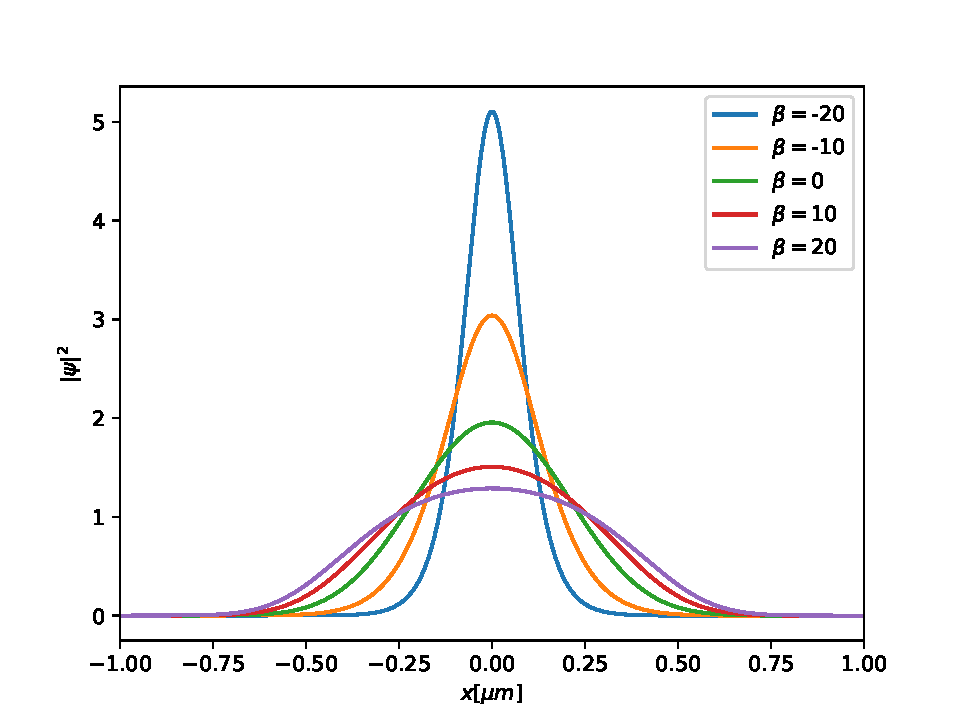
\includegraphics[width=\columnwidth]{graphics/stateAnalysis/GroundstateBeta.pdf}
	\end{subfigure}
	\begin{subfigure}{\columnwidth}
		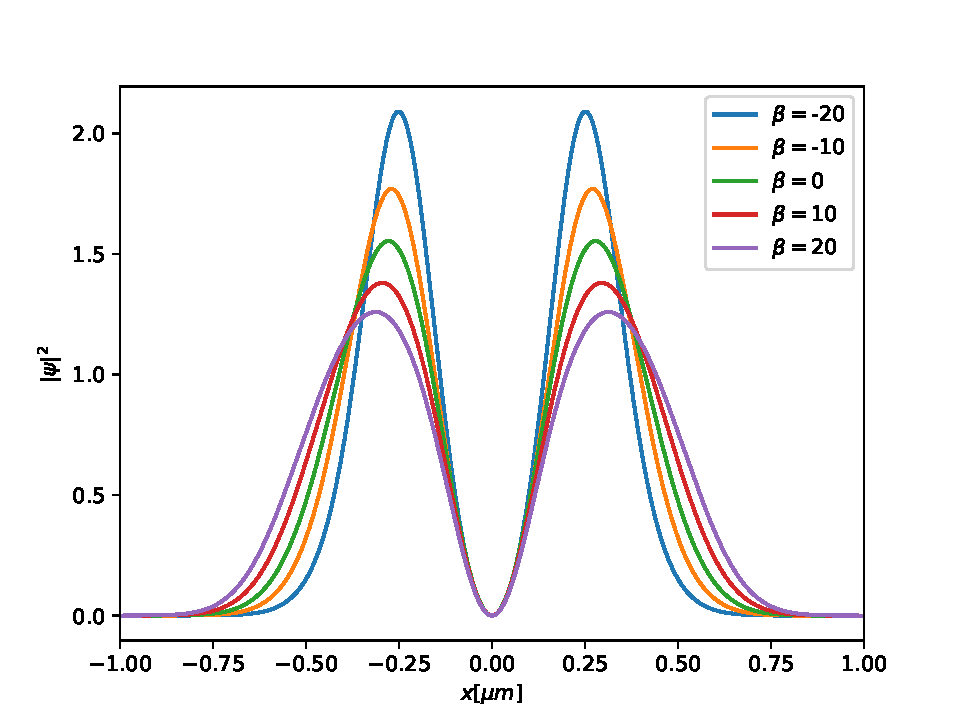
\includegraphics[width=\columnwidth]{graphics/stateAnalysis/ExcitedstateBeta.pdf}
	\end{subfigure}
	\caption{\textbf{Top:} Ground states of a BEC in the quartic trapping potential seen in Eq. \eqref{eq:quartic-potential} with $u(t)=0$ shown for different self interaction ($\beta$) strengths from Eq. \eqref{eq:Hbec}. \textbf{Bottom:} First excited state of the same system. Notice that the state grows in size when $\beta > 0$ and shrinks when $\beta < 0$. Potential parameters are found in Appendix \ref{App:System-params} under system \textit{B1}, here with $n_{\text{points}}=1024$.}
	\label{fig:BECstates}
\end{figure}

We attempt to excite the BEC from its ground state to first excited state using a control function, usually denoted $u(t)$. The control function describes how the potential evolves in time. A simple example of this is could be that $u(t)$ could describe how a quartic potential is displaced over time:
\begin{equation}
	V(x, u(t)) = a(x-u(t))^2 + b(x-u(t))^4
	\label{eq:quartic-potential}
\end{equation}
While it is not hard to write out \textit{some} control function, it is much more difficult to find a control that succesfully excites the initial state into the desired state. To quantify how well a given control function has performed, one can calculate the \textit{fidelity} $\mathcal{F} = | \langle \psi_D | \psi \rangle |^2$ to calculate the overlap between the two states $\ket{\psi}$ and $\ket{\psi_D}$, where $\ket{\psi}$ is the current state and $\ket{\psi_D}$ is some desired state. Thus, the fidelity $\mathcal{F}$ is a number between $0$ and $1$, where $0$ means that there is no overlap between the 2 states and $1$ means that the states are identical. Usually values of $0.99$ and above are set as the benchmark that a control function must satisfy. For plotting purposes it is more convenient to instead show the \textit{infidelity} $1-\mathcal{F}$ on a logarithmic scale to illustrate how well different control functions performed.\\

Since it can be very difficult to find a control function that is capable of reaching $\mathcal{F} \geq 0.99$, it is often useful to \textit{optimize} an initial control function (called a ``seed'' in this case) using different kinds of optimization algorithms. These optimization algorithms are, given enough time, usually capable of optimizing a seed into a control that can reach much higher fidelities. Regardless of which optimization algorithm is used, one must first define the optimization \textit{problem}, which is a function that the given algorithm will attempt to minimize. We define this problem as \cite{JensJacobPhDThesis} 

\begin{equation}
	\min J(u) = \frac{1}{2}(1-| \langle \psi_{t} | \psi(T) \rangle|^2) + \frac{\gamma}{2} \int_{0}^{T} \dot{u}^2 \text{d}t
	\label{eq:state-to-state}
\end{equation}
where $\psi_{t}$ is the target state, $\psi(T)$ is the final state evolved with the control $u(t)$ to final time $T$. The first term minimizes infidelity and the second term penalizes rapid fluctuations of the control function that can be challenging to implement experimentally. $\gamma$ is called the regularization factor and is usually on the order of $10^{-4}$ to $10^{-6}$. Additionally, a third \textit{boundary} term can be added to Eq. \eqref{eq:state-to-state} with a factor $\sigma$ which penalizes controls with values outside a defined interval $\{x_{lower}, x_{upper}\}$.\\

The optimization algorithm \proc{Grape} (\textbf{Gr}adient \textbf Ascent \textbf Pulse \textbf Engineering) \cite{KHANEJA2005296} is available to use in both Quantum Composer and the QEngine. \proc{Grape} works by calculating the gradient of $\mathcal{F}$ with respect to each point of a given control function on the discretized time scale 
\begin{equation}
	\vec{\nabla}_{\vec{u}} \mathcal{F}[\vec{u}]
\end{equation}
where $\vec{u} = (u(t_0), u(t_1) ... \,, u(T))$. When this calculation is done, $\proc{Grape}$ takes a step of size $\alpha_k$ such that the new discretized control function becomes
\begin{equation}
	\vec{u}_{k+1} = \vec{u}_{k} + \alpha_k \vec{\nabla}_{\vec{u}} \mathcal{F}[\vec{u}]
\end{equation}
such that $\mathcal{F}[\vec{u}_{k+1}] \geq \mathcal{F}[\vec{u}_{k}]$. This process is continued until some convergence criterium is fulfilled, e.g. a target threshold $\mathcal{F}[\vec{u}_{k}] \geq \mathcal{F}_{target}$, a maximum number of iterations $k \leq N$ or until the step size $\alpha_k$ becomes too small. \\

%TODO Expand theory on what Group and dGroup does and how they compare to Grape
Two other optimization algorithms are available to use in the QEngine: \proc{Group} and d\proc{Group} (dressed \proc{Group}). Where \proc{Grape} is a relatively simply gradient ascent algorithm, these two attempt to combine the local optimization that \proc{Grape} does with a global search for promising regions in the fidelity landscape \cite{GroupPaper, QEngine}. 
Note that this does not mean that an optimized seed will always be able to reach $\mathcal{F} \geq 0.99$. One particular hindrance is the \textit{Quantum Speed Limit} (QSL). This speed limit refers to the upper bound of how fast a state is able to evolve in time \cite{Deffner_2017}. This speed limit is (not surprisingly) dependent on the individual system examined and in the context of the Shake Up challenge, it refers to the minimum time required to evolve from the initial state into the target state with a fidelity of at least $\mathcal{F} \geq 0.99$. \\

The challenge was explored in Quantum Composer by creating different systems and control functions and optimization parameters. The control functions themselves were varied and explored, along with the control duration $T$ and the \proc{Grape} optimization parameters $F_{target}$, $N$, $\gamma$ and $\sigma$.
%TODO For next iteration write about control lanscape stuff using this citation \cite{doi:10.1142/S0219025713500215}

\section{Quantum Composer}\label{sec:Composer}
Quantum Composer is an educational tool for visualizing the behavior of a quantum mechanical system  \cite{ahmed2020quantum}, either statically or as the system evolves in time. To do this, one combines building blocks (nodes) containing the various components (like a potential $\hat{V}(x)$) to build new nodes (like a Hamiltonian $\hat{H} = \hat{T} + \hat{V}$). From there, one can build a wave function from a superposition of $\hat{H}$ eigenstates using one type of node and connect it to a plotting node to have the state, its norm-square and other relevant quantities visualized. The system can be evolved in time using a time node. The use of Composer in this report can be grouped into three overall groups: System setup, \proc{Grape} optimization and simulation. These groups and what they entice has been visualized in Fig. \ref{fig:workflow-composer}. 

\begin{figure*}
	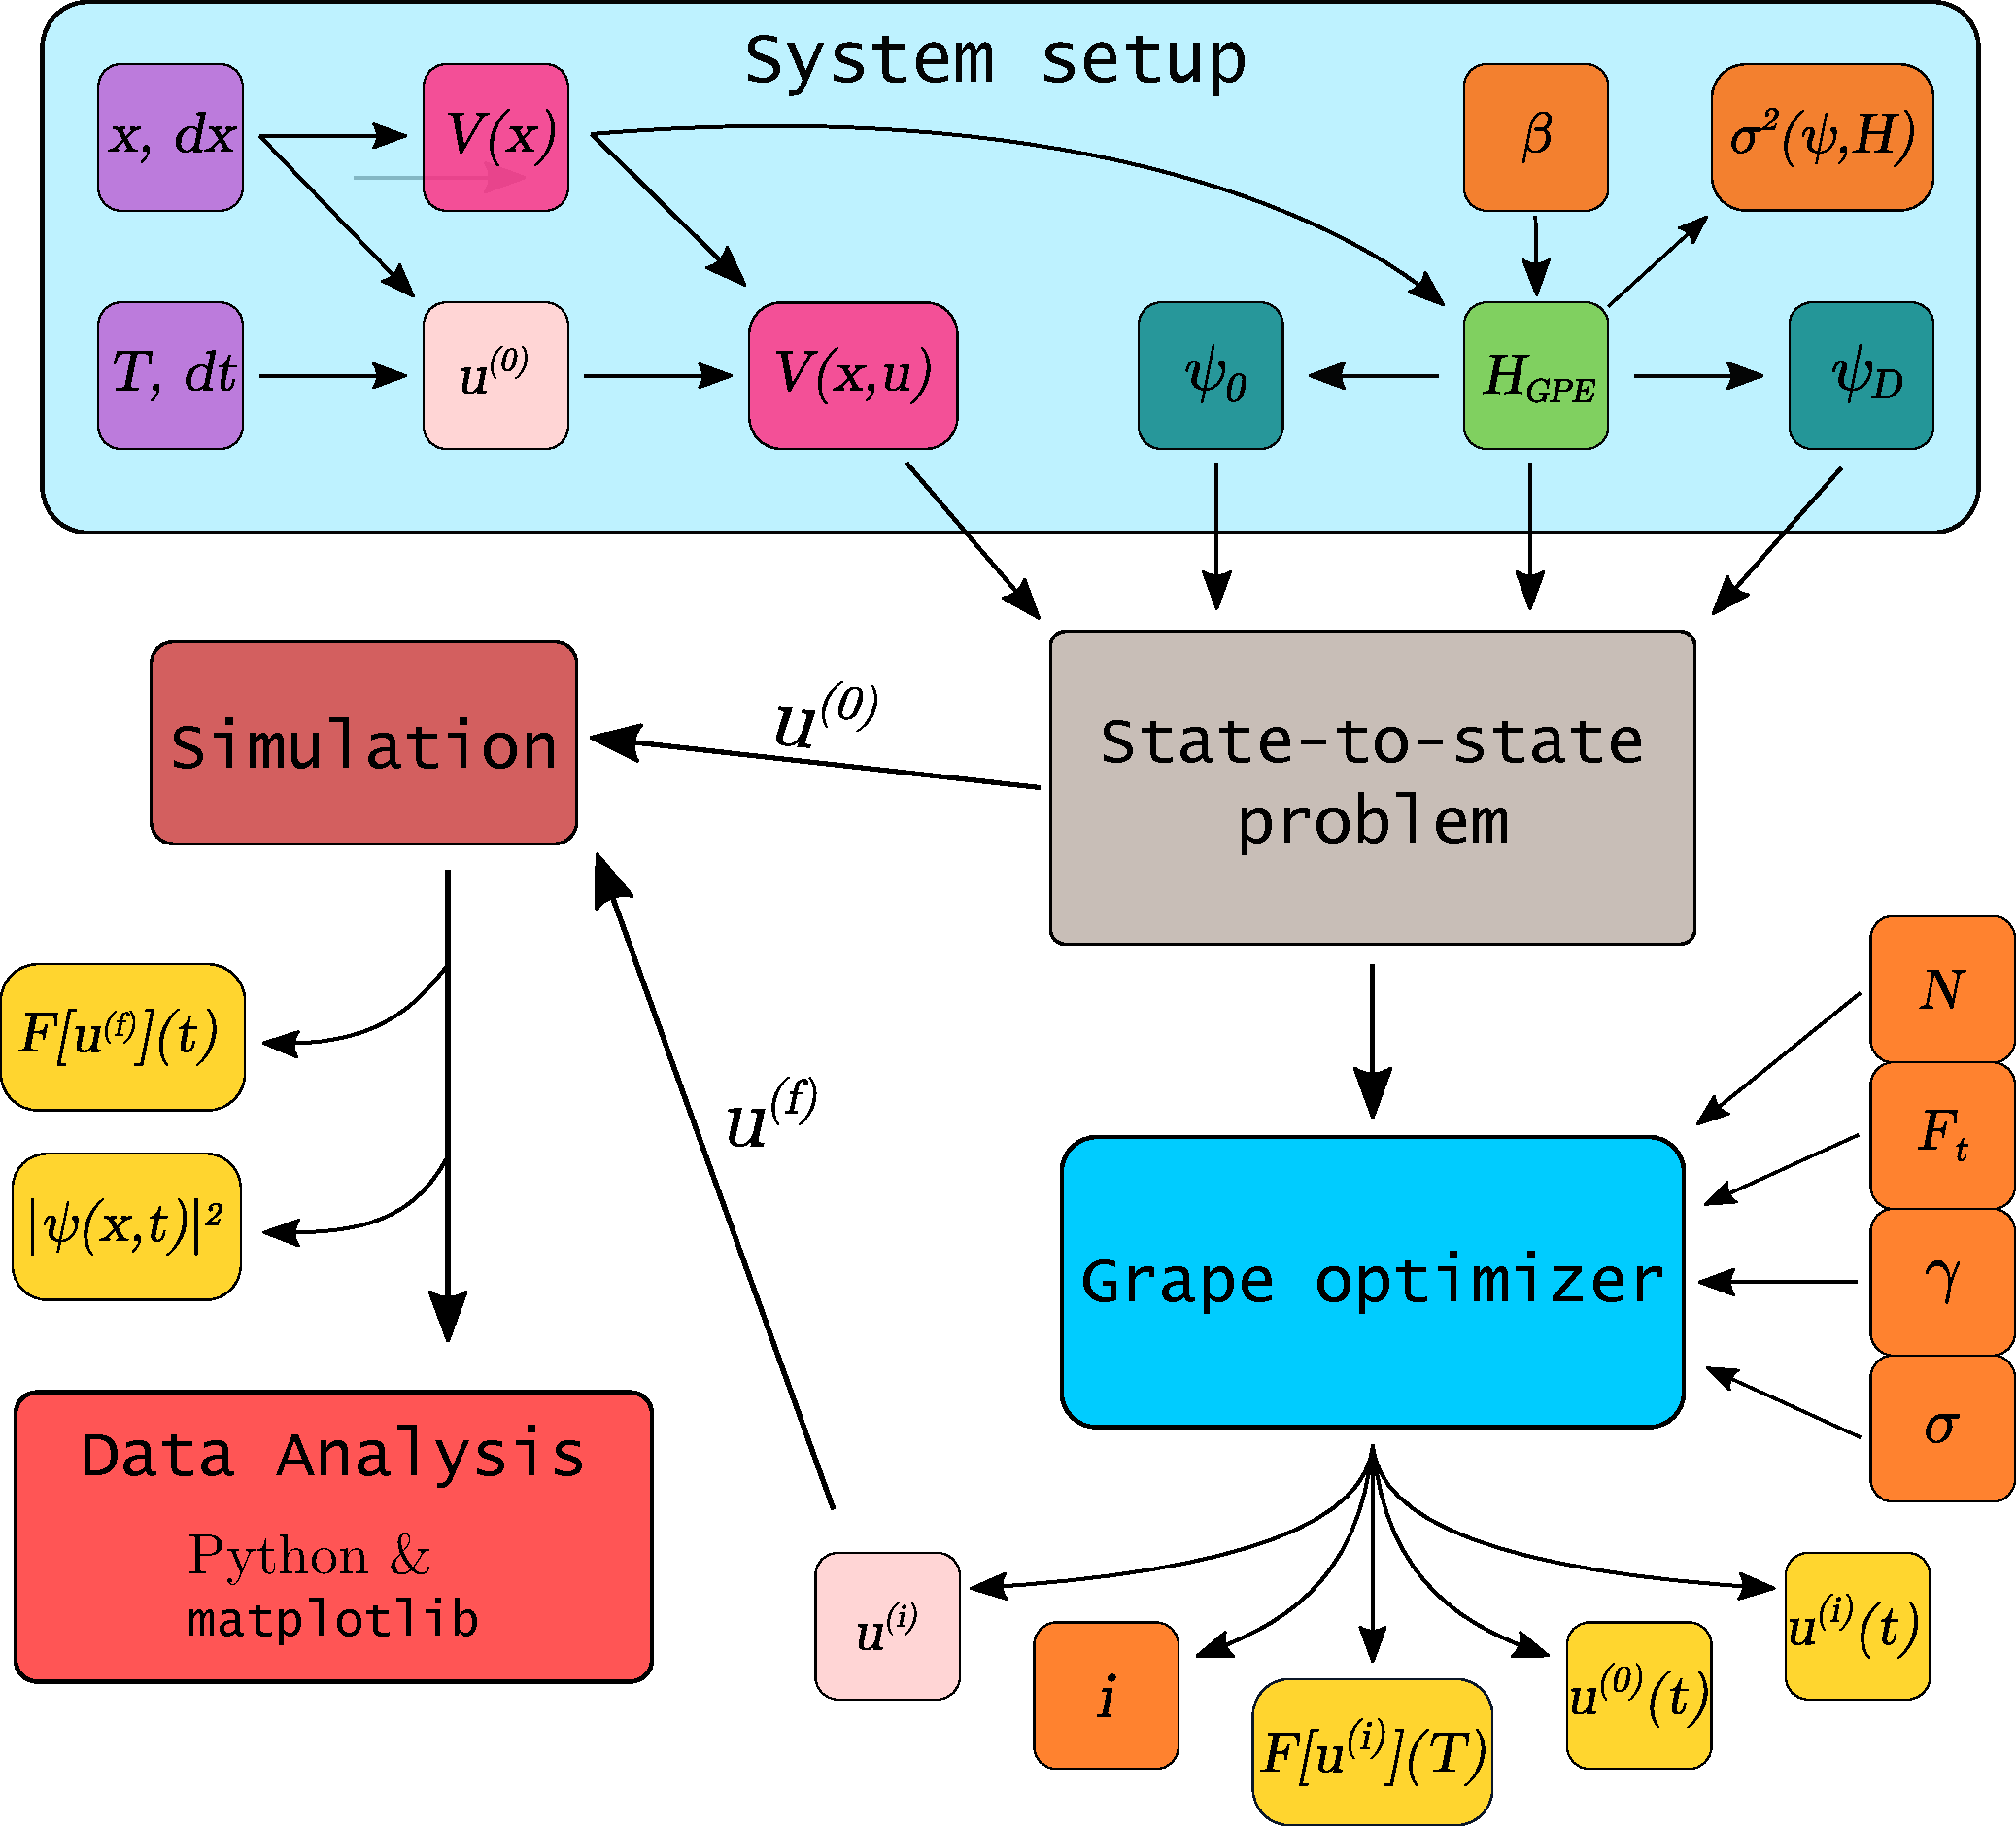
\includegraphics[width=0.75\textwidth]{graphics/composerScreens/workflow-v2.pdf}
	\caption{Diagram illustrating the workflow of using Quantum Composer. The different phases of working are illustrated with the \texttt{Phase nodes}, which depend on a number of smaller nodes. Nodes are colored by the type of data they represent, e.g. scalars are orange, graphs are yellow, etc.. Arrows indicate dependencies on other nodes. Note that a node in the diagram does not necessarily translate directly to a node in Composer, although many do.}
	\label{fig:workflow-composer}
\end{figure*}

To simulate a quantum control problem, one first has to set up a system that describes the problem. This includes choosing boundaries of the Hilbert space and discretizing the space into a number of points. It also includes things like describing the potential of the system and the time interval $(t_0, T)$. Specifically for quantum control problems it also involves defining how the potential depends on one or multiple control functions and how these are defined. From these steps, it is then possible to build the Hamiltonian of the system and from that we can create wave functions, in particular $\psi_0$ (the initial state, in this case the ground state of the BEC) and $\psi_D$ (the desired/target state, in this case the first excited state) that are relevant for a quantum control problem.


It is then possible to optimize the initial control function using \proc{Grape}. The optimization procedure requires a number of arguments, some optional ($\gamma$ and $\sigma$), others required ($N$ and $F_T$). The control function will then be updated until a convergence criteria is reached, after which \proc{Grape} outputs the optimized control function. In Composer it is possible to map the fidelity of the current and previous control iterations to show how fidelity improves as \proc{Grape} iterates. Likewise, it is also possible to plot the initial and current control function to see how they differ. A screenshot from Composer showing how this optimization procedure is set up can be seen in Fig. \ref{fig:composerScreens}.

\begin{figure*}
	\centering
	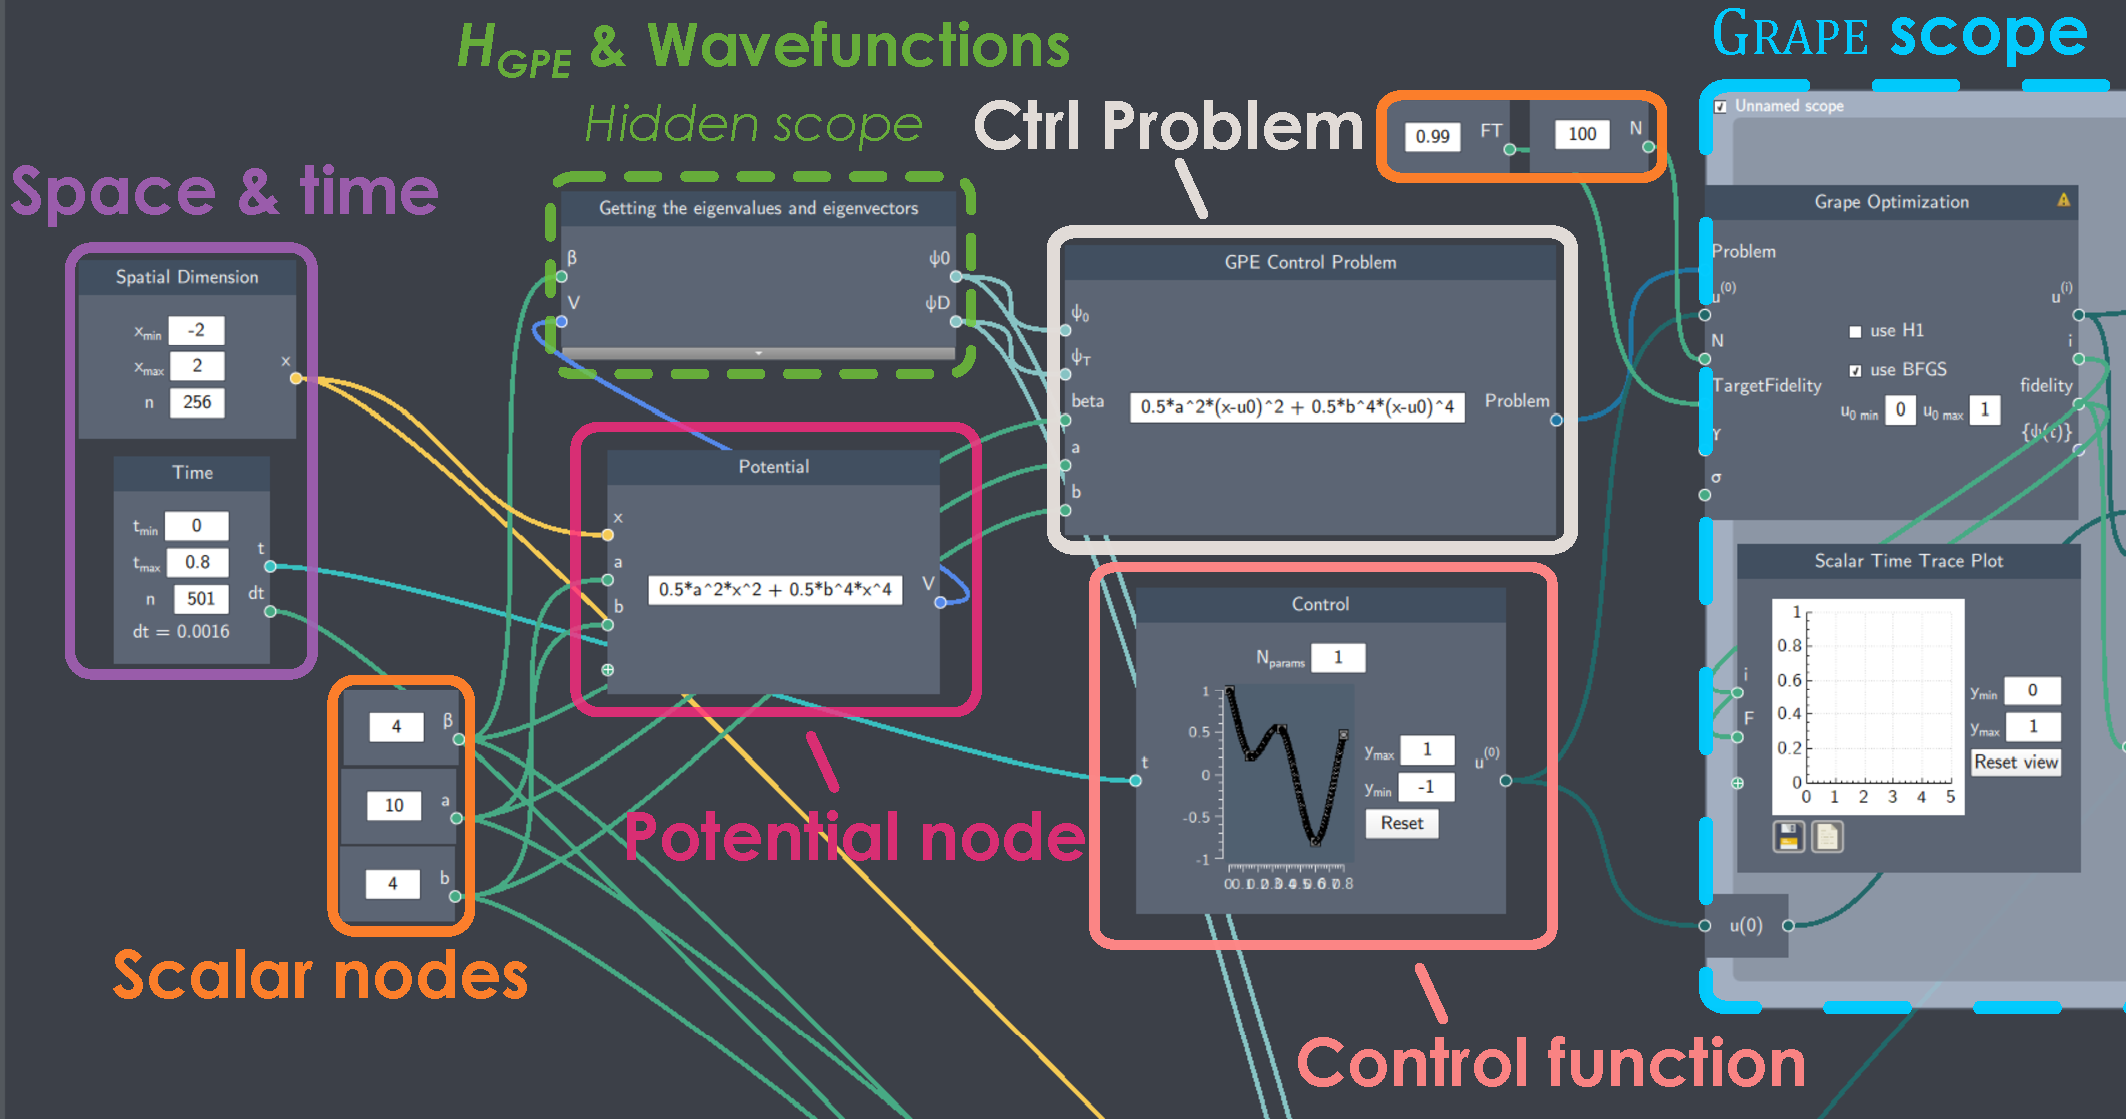
\includegraphics[width=\textwidth]{graphics/composerScreens/screenshot-v2-highlights.pdf}
	\caption{Screenshot from Quantum Composer partially showing a flowfile that optimizes a control function using \proc{Grape}. The nodes and scopes follow the same color scheme as in Fig. \ref{fig:workflow-composer}. Not shown is the scope where the optimized control is simulated and the resulting $\mathcal{F}(t)$ and $|\psi(x,t)|^2$ graphs are generated.}
	\label{fig:composerScreens}
\end{figure*}

When the system is simulated, it is possible to analyze the wave function at the current point in time. Thus we are able to calculate and visualize different variables in our system as they are being simulated. This includes calculating the fidelity $F$ as a function of time, but we can also plot how our wave function evolves in time by mapping out $|\psi(x,t)|^2$. When the simulation is finished, the final fidelity $F(T)$ can be recorded.


The data presented in Composer, in most cases, cannot be saved directly through the program, but must instead be manually written to a separate text file. This file containing data can then be further analyzed and plotted. In this case it is done using \proc{python} and its plotting module \texttt{Matplotlib.pyplot}.


\section{Results}\label{sec:results}
\subsection{Numerical limitations}\label{subsec:numericalLimitations} 
\subsubsection{Spatial resolution \& performance}
% Compare grid resolution errors
One obvious source of numerical inaccuracies is the resolution of the quantized Hilbert space one uses. Throughout the report, the spatial grid was divided into $256$ points. We can compare this resolution to other resolutions by calculating the difference between a high resolution wave function with $1024$ points and lower resolution wave functions. This difference between the different resolutions for the ground state can be seen in Fig. \ref{fig:groundstateGrid}. As can be seen in the figure we find that the lower the resolution of a wave function is, the bigger the difference between that wave function and a higher resolution one. \\
\begin{figure}
	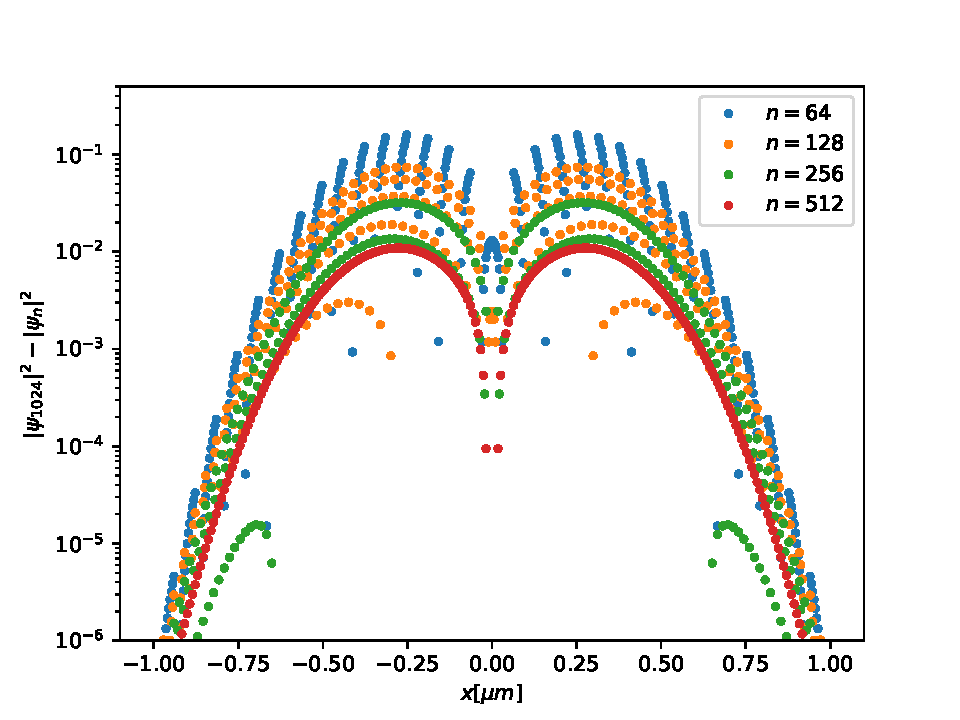
\includegraphics[width=\columnwidth]{graphics/stateAnalysis/GroundstateGrid.pdf}
	\caption{Difference between different resolutions of the initial wave function compared to a higher resolution wave function with $n = 1024$. Lowering the spatial resolution results in increasingly larger error.}
	\label{fig:groundstateGrid}
\end{figure}

% Relate this to time consumption to explain why we dont do use the 1024 size but instead the 256
Considering this, one would think that it would always be better to use as high spatial resolution of a given system as possible. This would of course be true if we had access to unlimited computational power. We instead have to balance the desire for a high spatial resolution and more accurate wave functions against the increased time it takes to do calculations for a higher dimension Hilbert space. As an example of this increased calculation time, a system was set up as described by System \textit{B1} seen in Appendix \ref{App:System-params}, with additional parameters: $\beta = 4$, $u(t)=0.5 \cos(2\pi t/T)$ and $T=0.8$. This system was then optimized for 100 iterations using \proc{Grape} before the system was simulated with the optimized control function. The results can be seen in Fig. \ref{fig:performanceTime}. This result confirms that choosing a grid resolution of $256$ points gives us a high accuracy compared to lower resolutions while also keeping performance time low.

\begin{figure}
	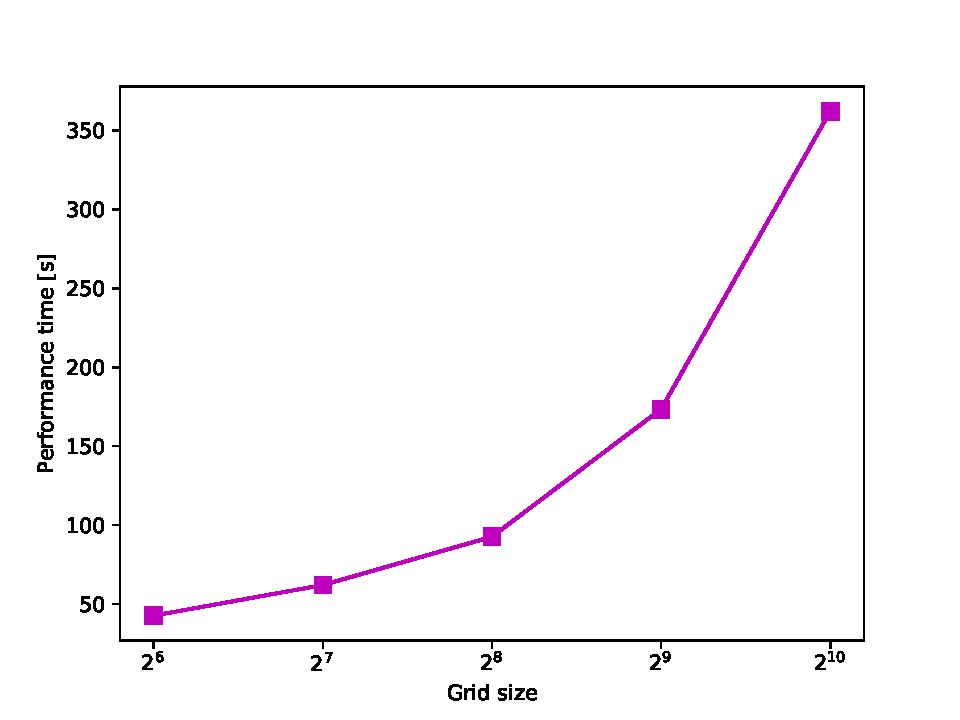
\includegraphics[width=\columnwidth]{graphics/stateAnalysis/PerformanceTime.pdf}
	\caption{The time it takes for Quantum Composer to solve a specific problem described in the main text as a function of the spatial grid resolution. The grid size of $n=256=2^8$ was found to be optimal in terms of the accuracy vs. performance time.}
	\label{fig:performanceTime}
\end{figure}

\subsubsection{Spatial limitations of controls}\label{subsubsec:spatial-limitations-of-controls}
One could think, after having defined a spatial grid between 2 points $\{x_{min},x_{max}\}$, that any given control function is then able to utilize the entirety of this grid. While the control function itself does not cause problems by roaming near the edges of the simulated space, the state being controlled does indeed cause big problems if parts of the wave ``spill'' out over the edge of the defined space. This phenomenon is demonstrated on Fig. \ref{fig:statePlots}, where the left state spills outside the space and ``breaks'' the simulation while the right shows a regular simulation. This can also happen when the control accelerates the state so rapidly that it can't slow the state down and ``catch'' it again. \\

\begin{figure}
	\begin{subfigure}{0.45\columnwidth}
		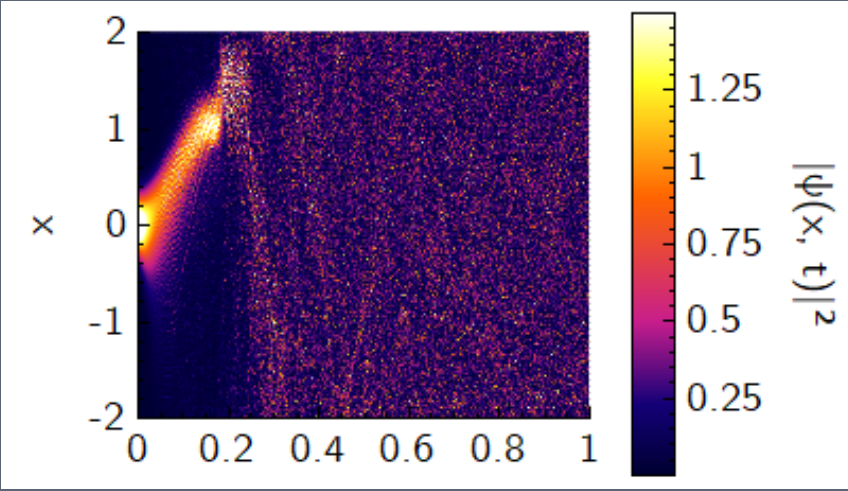
\includegraphics[width=\columnwidth]{graphics/clustering/QM2Clusteringk4A04T06178-2.PNG}
	\end{subfigure}
	\begin{subfigure}{0.45\columnwidth}
		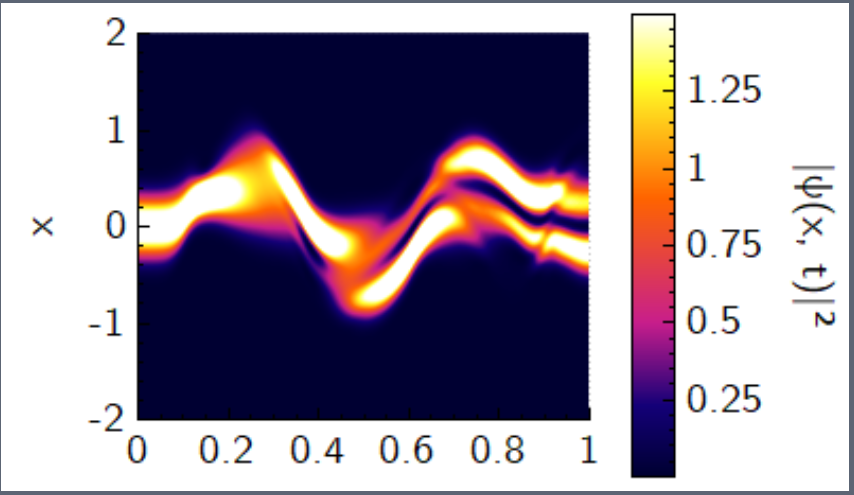
\includegraphics[width=\columnwidth]{graphics/clustering/QM2Clusteringk5A015T07475-2.PNG}
	\end{subfigure}
	\caption{Comparison of the state evolution for a numerically broken state (left) and a numerically working state (right). On the first axis is normalized control time and on the second axis position in $\mu$m.}
	\label{fig:statePlots}
\end{figure}

To further investigate this problem, a simulation with no optimization was set up. The purpose of these simulations were not to find the highest fidelity, but to find the highest amplitude $A$ of the control function
\begin{equation}
	u_{amplitude}(t) = A \sin(3\pi t/T)
	\label{eq:control-amplitude-variation}
\end{equation}
possible, where the state did not spill over the space edges and break. For comparison purposes, this was experiment was repeated for three different spatial boundaries: $x\in \pm \SI{2}{\micro\meter}, \pm \SI{4}{\micro\meter}$ and $\pm \SI{6}{\micro\meter}$. The potential and self interaction strength $\beta$ is noted in Appendix \ref{App:System-params} under \textit{Composer impl. of QM2 Shake up}. The results are shown in Fig. \ref{fig:amplitude-variations}, which consists of 2 sub figures. The upper figure shows that for control durations below $1 \text{ ms}$, the highest amplitudes attainable are found in grids with boundaries $x\in \pm \SI{4}{\micro\meter}$ and for higher durations the most suitable bounderies are $x\in \pm \SI{6}{\micro\meter}$. The lower sub figure shows the ratio between the maximum amplitude found that the space boundaries. This shows that in terms of amplitude relative to space size, the 3 grid sizes each outperform the others such that increasing boundaries increases with control duration. 

These results can be useful in cases where Composer is used as an exploration tool prior to an experiment. If the experimental boundaries are around $\pm \SI{2}{\micro\meter}$, it seems advantageous to use a boundary slightly larger for simulations with small timescales. This ensures that it is possible to fully explore the relevant control space.

It should be noted that while it has been demonstrated that it can be beneficial to increase the grid spacing, it comes at the cost of increasing the variance of important states ($\psi_0$, $\psi_D$). These settings should ideally be tuned to each simulation since it is possible to prioritize the trade off between performance and accuracy to a great extend. This trade off confirms what figures \ref{fig:groundstateGrid} and \ref{fig:performanceTime} demonstrate, discussed in the previous subsection.  

\begin{figure}
	\begin{subfigure}{\columnwidth}
		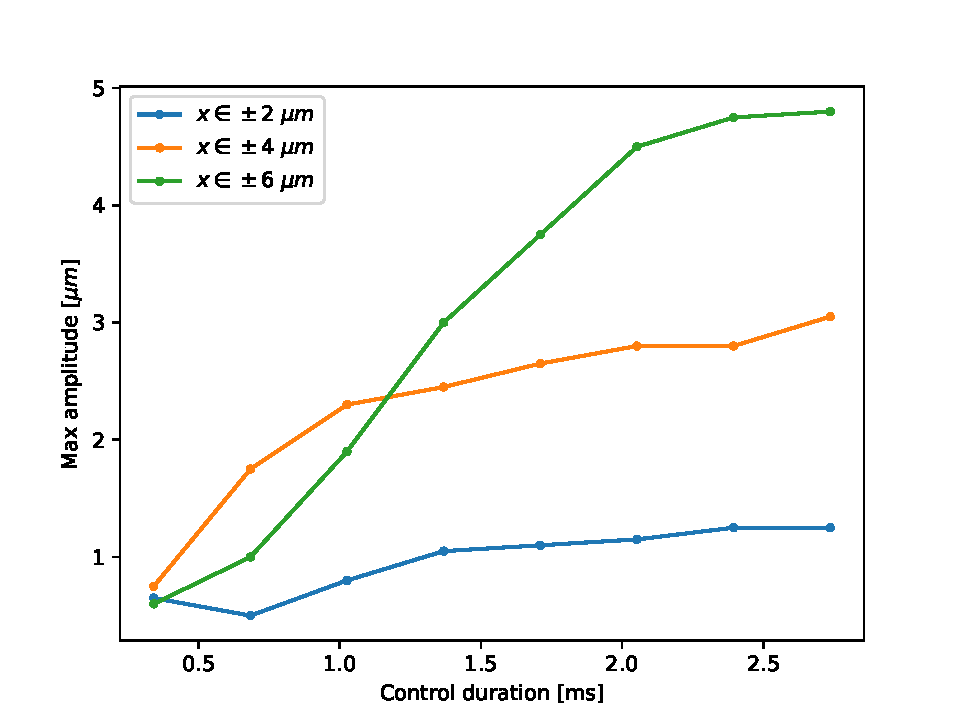
\includegraphics[width=\columnwidth]{graphics/numerical-limits/amplitude-variation.pdf}
	\end{subfigure}
	\begin{subfigure}{\columnwidth}
		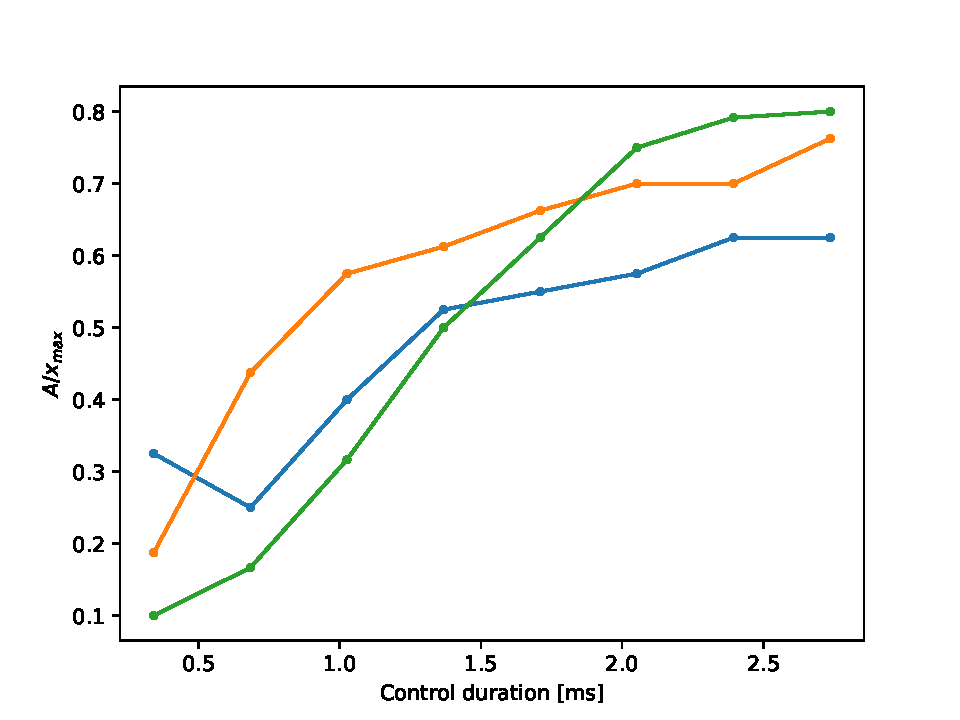
\includegraphics[width=\columnwidth]{graphics/numerical-limits/amplitude-variation-relative.pdf}
	\end{subfigure}
	\caption{Maximum possible amplitude $A$ in the control function in Eq. \eqref{eq:control-amplitude-variation} where the simulation does not break, simulated on 3 different grid sized $x\in \pm 2, \pm 4, \pm 6$. \textbf{Top:} Value of $A_{max}$ as a function of control duration $T$. \textbf{Bottom:} Maximum amplitude relative to the maximum grid value. Bigger spatial boundaries makes the a bigger portion of the control space available for exploration. In some cases it seems viable to change the spatial boundary size depending on the control duration of the problem in order to maximize the possible control amplitude.}
	\label{fig:amplitude-variations}
\end{figure}
%The dip of the $\pm 2$ curve (blue) is caused by the state being accelerated towards the boundary so quickly that it can't be ``caught'' again. Not sure if relevant

\subsubsection{Eigenstates \& eigenvalues}

In order to obtain accurate results when making these computations, one has to ensure that the states that are analyzed are described within acceptable numerical accuracy. We can ensure that we are working with the ground state as our initial state in Composer by calculating the variance of our initial state with respect to the Hamiltonian operator. The variance of a state with respect to an operator $\hat{\mathcal{O}}$ is given by
\begin{equation}
	\text{Var}(\psi, \hat{\mathcal{O}}) = \langle \psi | \hat{\mathcal{O}}^2 | \psi \rangle - \left(\langle \psi | \hat{\mathcal{O}} | \psi \rangle\right)^2
\end{equation}

This gives us a numerical estimate of how ``close'' our initial state is to the actual ground state of $\hat{H}_{GPE}$ since
\begin{equation}
	\psi \text{ is an eigenstate of } \hat{H}_{GPE} \iff \textsc{Var}(\psi, \hat{H}_{GPE}) = 0
\end{equation}

The way the energy spectrum of $\hat{H}_{GPE}$ is calculated is not trivial \cite{QEngine}, but the variance can generally be reduced by adjusting different parameters of the system or Composer file, e.g. spatial dimension $x$ or initial conditions for the $H_{GPE}$ spectrum node. Despite these possible fixes, the numerical limitations of Quantum Composer become apparent as the shakeup problem is explored in increasingly greater details and limits and accuracy are pushed further and further. The following paragraphs describe areas where the numerical limitations are significantly limiting the exploration of certain aspects of this problem.\\

Composer was also used to show how the energy levels of the BEC energy eigenstates changed as the self interaction was varied. The energy levels were studied both for a BEC in a quadratic potential (\textit{System A1} in Appendix \ref{App:System-params}) and a quartic potential (\textit{System B1}). Figure \ref{fig:energyLevels} shows the how the energy levels of the 3 lowest energy eigenstates change with self interaction strenght. Below that it shows the energy spacing between these 3 levels for both potentials. 

Firstly note that Composer is only capable of calculating the second excited state with great uncertainty outside a narrow interval around $\beta = 0$. This uncertainty can be reduced slightly by changing initial parameter guesses in the spectrum generating procedure, but it is not reducible to negligible levels ($\leq 1$) as for the uncertainties of the other states shown.

It should be noted how the self interaction strength $\beta$ affects the spacing between the energy levels. For non-interacting and repulsive interactions between atoms we see that the spacing is still equally spaced. Due to the uncertainty of the 2nd excited state energy, we are unable to actually conclude if this behavior is true and so we can also say that these results indicate that the equal spacing also holds for repulsive BECs. This is not the case for BECs with attractive self interaction, where the energy spacing between the 2 lowest states rapidly increases compared to the spacing between the 2 highest states. This increase in spacing is so large that it even surpasses the considerable uncertainty of the difference between 1st and 2nd excited state. \\

\begin{figure}
	\begin{subfigure}{\columnwidth}
		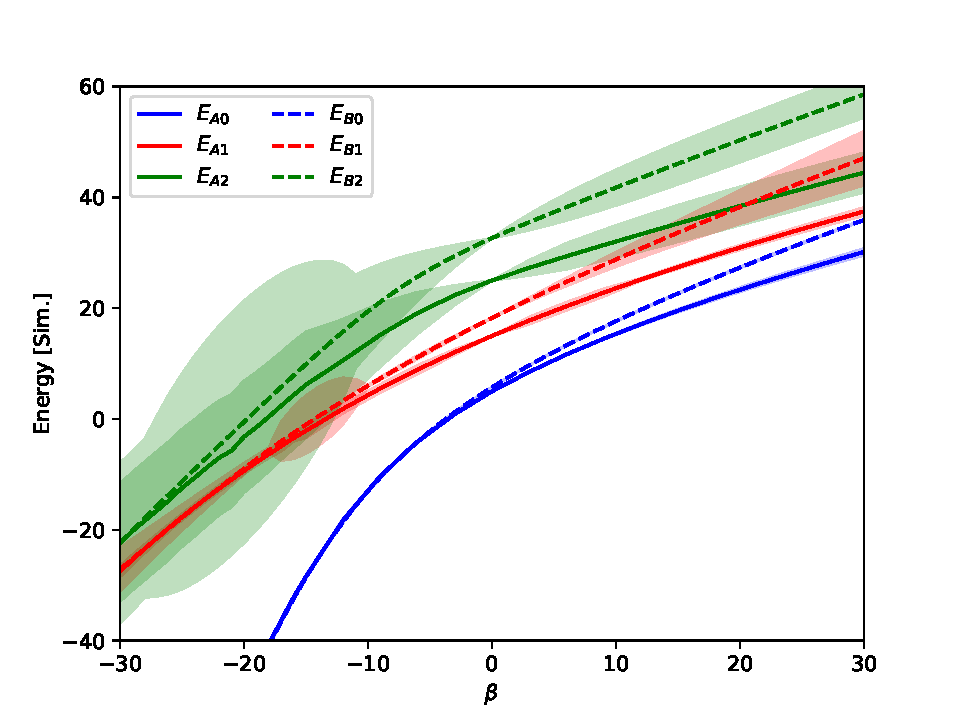
\includegraphics[width=\columnwidth]{graphics/stateAnalysis/Energylevels.pdf}
	\end{subfigure}
	\begin{subfigure}{\columnwidth}
		\includegraphics[width=\columnwidth]{graphics/stateAnalysis/EnergyDifference.pdf}
	\end{subfigure}
	\caption{\textbf{Top:} Energies of the ground state and first 2 excited states of a BEC with self interaction strength $\beta$ for a quadratic (full drawn lines) and quartic (dashed lines) potential with $u(t) = 0$. \textbf{Bottom:} Difference between state energies of the energies shown above. Uncertainties marked show the square root of the variance in both figures. Notice in particular that the equally spaced energy levels of the quardratic potential at $\beta=0$ remains somewhat equal as the interaction becomes more repulsive, while the distance grows rapidly with a more attractive self interaction.}
	\label{fig:energyLevels}
\end{figure}

\subsection{Harmonic potential optimization}
Due to the equally spaced energy levels of a quadratic potential, it is difficult to excite the state exclusively to the first excited state. It is likely that some part of the state is driven into higher excited states and so it is seemingly impossible to reach high fidelities with this kind of potential. Nonetheless, the nonlinear contribution to the GPE Hamiltonian seems to make it possible to improve the fidelity of control functions compared to the levels reachable for a single particle. In a quadratic potential different controls were optimized to estimate the highest reachable fidelity for this kind of potential as a function of the self interaction strength $\beta$. These controls were optimized with \proc{Grape} for $100$ iterations and the highest reachable fidelity was then noted. The potential parameters are described in Appendix \ref{App:System-params} under \textit{A1}. \\

The results can be seen in Fig. \ref{fig:HO}. As can be seen on the figure, it is actually possible to reach higher levels of fidelity for all measured values of $\beta \neq 0$ with control duration $T = 1$. The highest result shows that it is possible to improve the fidelity score with about $50\%$ compared to the reachable score of a single particle. One should also note that controls with duration $T=7.5$ do not perform as well as the other 2 shown durations. This is suspected to be caused by the long control duration allowing for states to be excited beyond the targeted first excited state, which the smaller control durations are not as susceptible to. Another explanation could be that the increased control duration makes the optimization landscape more complex and so more sensitive to the inital control that is being optimized on.

\begin{figure}[h]
	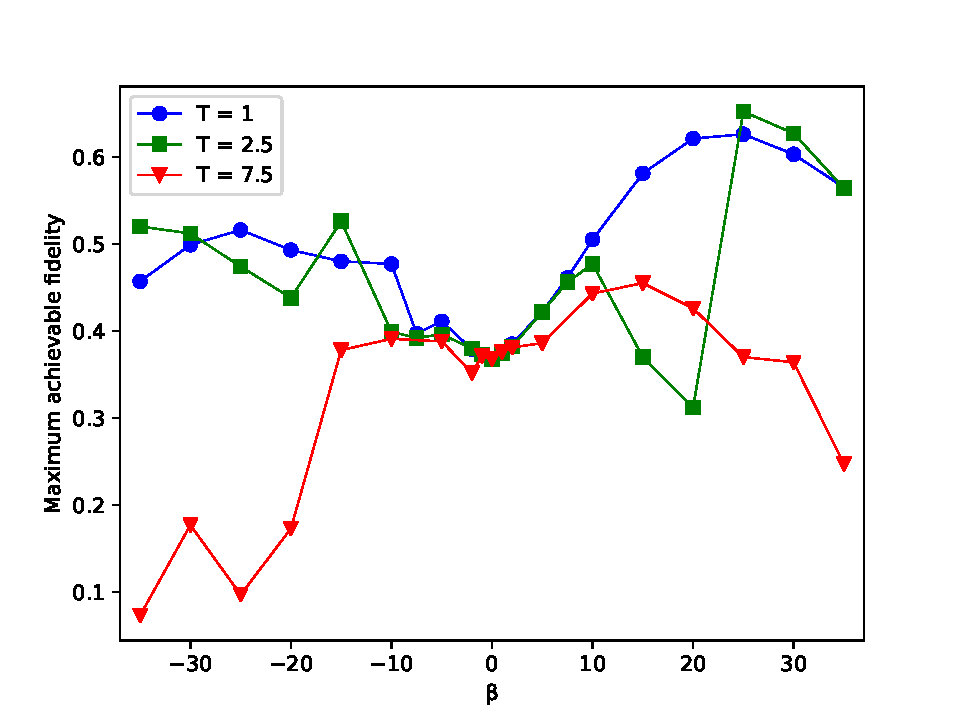
\includegraphics[width=\columnwidth]{graphics/exploration/betaTHO.pdf}
	\caption{The result of varying $\beta$ and $T$ for a BEC in the harmonic potential. There exist combinations where it is possible to achieve above $50\%$ higher fidelity compared to a single particle (at $\beta=0$), but many also combinations also perform worse than for a single particle.}
	\label{fig:HO}
\end{figure}
%TODO Test out if better results are reachable near T = 1

\subsection{Unoptimized BEC control in a quartic potential}
Through simulations it seems that BECs have very different dynamics compared to single particles. Without using $\proc{Grape}$, one can study how the similarity between single particles and BECs changes depending on the value of $\beta$. Keeping the control function and control duration the same, we find that what was a good solution for a single particle reaches a lower and lower fidelity as we change $\beta$ away from 0, but that it also reaches revivals with a higher fidelity compared to neighboring values. This behavior is shown in Fig. \ref{fig:beta} where the non-optimized control
\begin{equation}
	u_{\mathrm{non-opt}}(t)=0.12\cdot\sin(0.86\cdot \omega_{01} t)
	\label{eq:nonopt-control}
\end{equation} with final time $T=3.49$ was simulated for different values of $\beta$. The potential parameters are described in Appendix \ref{App:System-params} under \textit{B1}. We define $\omega_{01}$ to be the energy frequency between the ground and first excited state. This variation is not unexpected. The function in Eq. \eqref{eq:nonopt-control} was chosen because of its high fidelity score around $\beta=1$, but expecting this control function to perform well for the wide range of other systems (i.e. values of $\beta$) it is tested on would not be expected. While the behavior of similar systems is not vastly different, this small change to the system dynamics does mean that some systems will not reach a high fidelity at the final time, while others will. This can also be seen in Fig. \ref{fig:fidelityplot}, where the fidelity as a function of time has been plotted for 2 different interaction strengths. 
In conclusion, using a single, non-optimized control for a broad range of systems is not viable, as success boils down to timing whether or not the control terminates at a high fidelity.

\begin{figure}[h]
	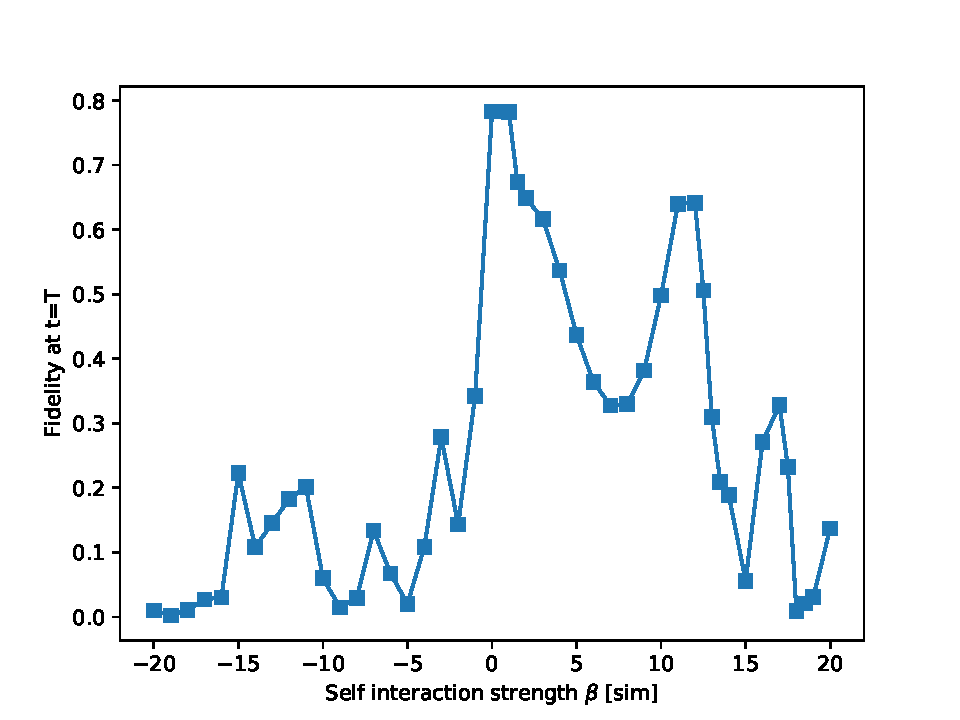
\includegraphics[width=\columnwidth]{graphics/exploration/nonOptBeta.pdf}
	\caption{Fidelity of a non-optimized solution for different values of $\beta$ in the quartic potential from Eq. \eqref{eq:quartic-potential} with $u(t) = 0$. The fidelity drops off as $\beta$ is moved away from $0$, but there are also revivals where the fidelity reaches a local peak. These revivals can be explained by looking at the fidelity as a function of time, two examples of which are shown in Fig. \ref{fig:fidelityplot}.}
	\label{fig:beta}
\end{figure}

\begin{figure}
	\begin{subfigure}{0.45\columnwidth}
		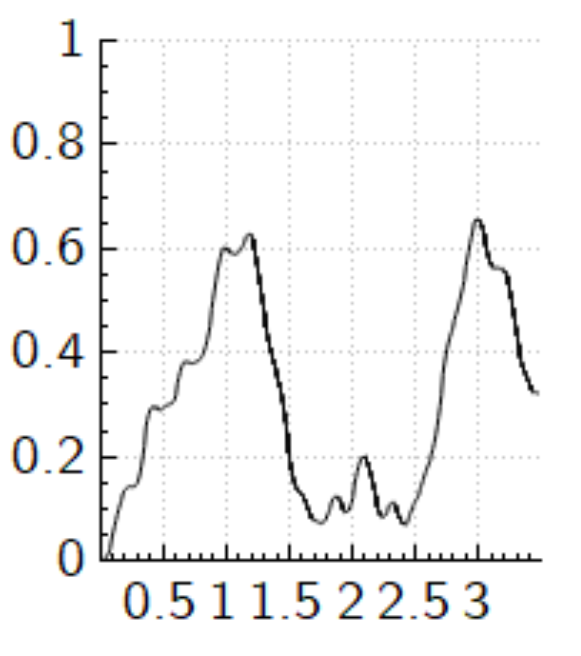
\includegraphics[width=\columnwidth]{graphics/exploration/betaNonOptFidelityBeta7.PNG}
	\end{subfigure}
	\begin{subfigure}{0.45\columnwidth}
		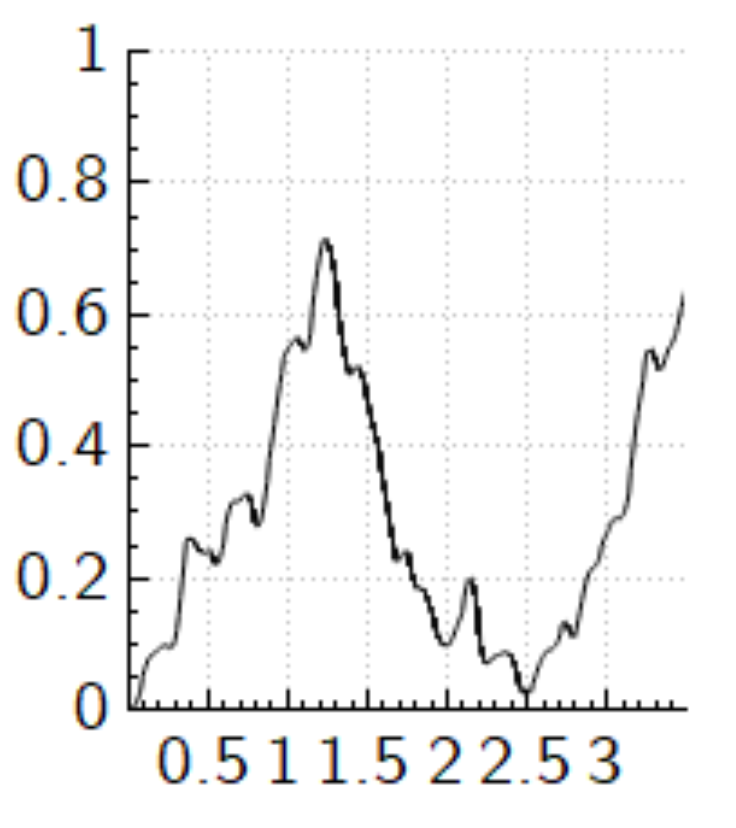
\includegraphics[width=\columnwidth]{graphics/exploration/betaNonOptFidelityBeta12.PNG}
	\end{subfigure}
	\caption{Fidelity as a function of time for the control function in Eq. \eqref{eq:nonopt-control} for two different values of $\beta$. \textbf{Left:} $\beta=7$. \textbf{Right:} $\beta=12$. As can be seen, the overall trend is the same for the 2 systems and so it becomes a matter of ``timing'' the final time to reach a higher fidelity if one refrains from using \proc{Grape} to optimize controls.}
	\label{fig:fidelityplot}
\end{figure}

\subsection{Quantum speed limit}
It was attempted to estimate the Quantum Speed Limit for this control problem and its dependence on the interaction strength of the BEC, $\beta$. The system parameters used are described under \textit{System B1} in Appendix \ref{App:System-params}. The methods for determining seeds are discussed in section \ref{sec:strats}. The seeds chosen were then optimized for 100 iterations in order to estimate the duration above which optimized controls reach a fidelity of $0.99$. The resulting estimates of the QSL for different values of $\beta$ can are shown in Fig. \ref{fig:QSL}. Notice how it seems that the speed limit is lower for attractive BECs and increasingly higher for increasingly more repulsive BECs. It was not possible to estimate the QSL for values of $\beta$ below $-10$ or above $25$, since no control function could be optimized to $0.99$ within 100 iterations. The speed limit was found to be lowest at the values $\beta\in\{-5,0,0.5,1\}$ where the speed limit was estimated to $0.63\mu_{time} \approx 0.86\text{ms}$.\\

\begin{figure}[h]
	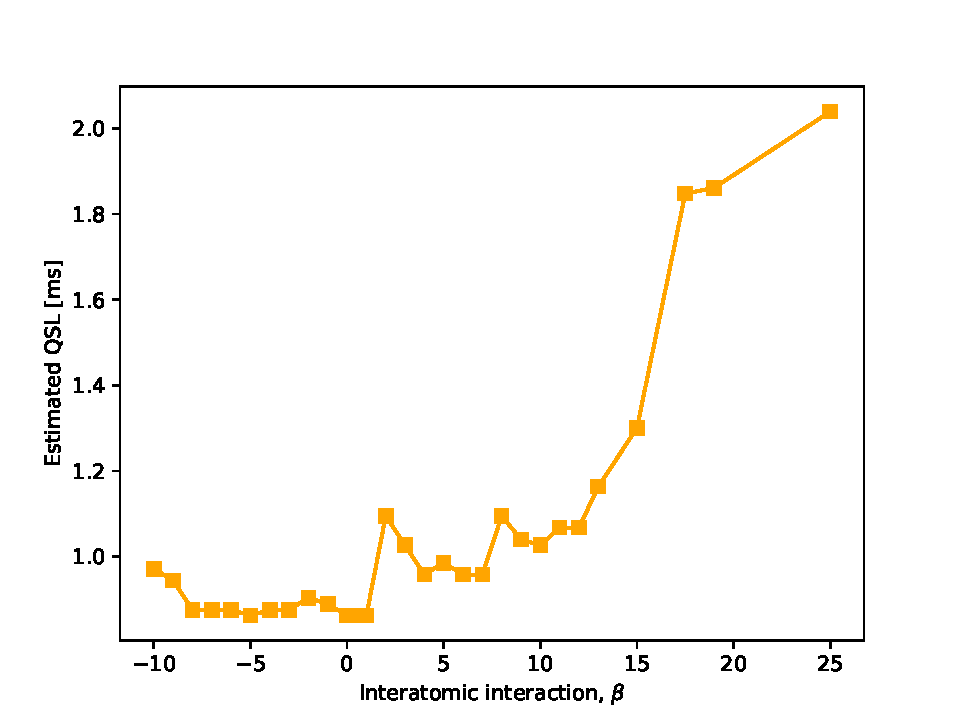
\includegraphics[width=\columnwidth]{graphics/exploration/QSL.pdf}
	\caption{The estimated Quantum Speed Limit for a BEC in a quartic potential as a function of $\beta$. The speed limit was found to generally increase for $\beta>0$, while it was found to be around the same value for $\beta\leq0$. Note that the highest speed limit found at $\beta=25$ was more than twice as high as the lowest found around $\beta \sim 0$.}
	\label{fig:QSL}
\end{figure}

\subsection{Optimizable boundaries of the BEC self interaction}\label{subsec:optimizable-boundaries-of-beta}

It is clear after having explored the behavior of BECs in different numerical setups that the behavior the BECs are not symmetric with respect to $\beta$. This is not unexpected, since the sign of $\beta$ constitutes whether the atom-atom interaction happening inside the BEC is repulsive($\beta>0$) or attractive ($\beta<0$) and so it would not be unjustified to say that the sign of $\beta$ describe entirely different species of bosons. Since attractive BECs have proven difficult to optimize on for $\beta<-5$, it was explored what the lower limit of $\beta$ would be with respect to reaching an optimizable fidelity of at least $0.99$. The results of this exploration is seen in Fig. \ref{fig:reachable_neg_betas}, where it can be seen that for values of $\beta<-10$ it is no longer possible to reach $F\geq0.99$. While this lower bound could be seen as a numerical limitation of Composer as discussed in Sec. \ref{subsec:numericalLimitations}, it is also relevant to consider that there exists a lower bound for how attractive a BEC can be before the atoms collapse in on themselves in a process known as a Bose-Nova \cite{Donley2001}.


\begin{figure}
	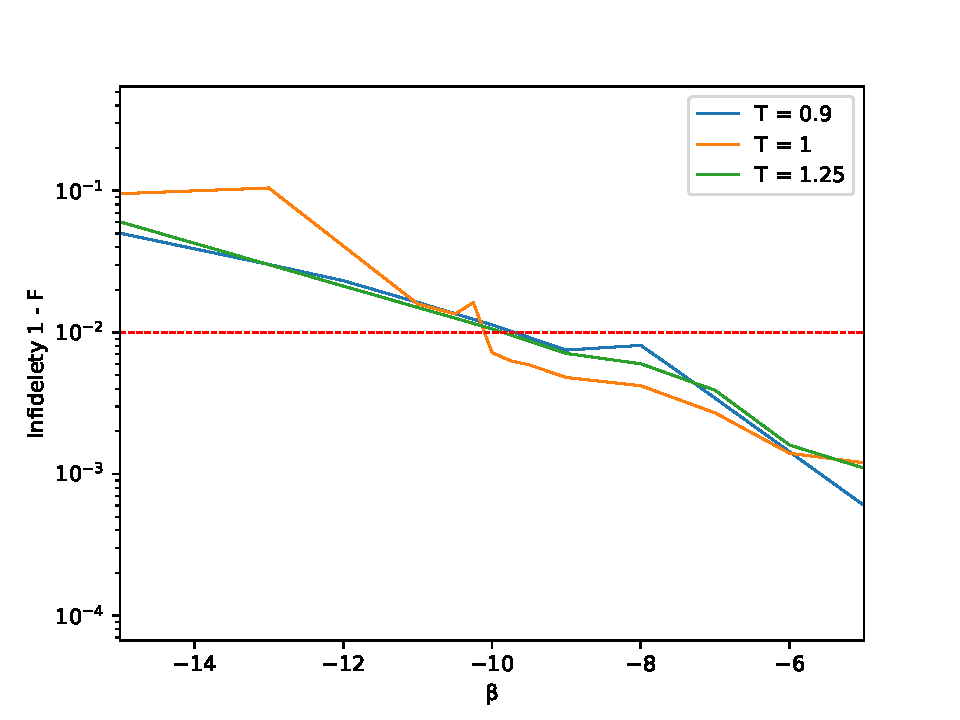
\includegraphics[width=\columnwidth]{graphics/exploration/reachable_neg_beta.pdf}
	\caption{Lowest reachable infidelities as a function of interatomic attraction $\beta$, shown for different timescales. It seems that $\beta=-10$ is the lower limit for reaching optimizable solutions $F\geq0.99$. This lower limit is, however, suspected to be caused by numerical inaccuracies. The red line marks where the fidelity of a control is $0.99$.}
	\label{fig:reachable_neg_betas}
\end{figure}

\begin{figure}
	\includegraphics[width=\columnwidth]{graphics/exploration/Reachable_Positive_betas.pdf}
	\caption{Similarly it is found that there is an upper bound to the self interaction strength, beyond which it is not possible to optimize beyond $\mathcal{F} \geq 0.99$. This upper bound seems to be inversely proportional to the control duration, as the results shown here suggests.}
	\label{fig:reachable_pos_betas}
\end{figure}

\subsection{Clustering of solutions}\label{subsec:composer-clustering}
The shakeup problem has also been studied in a recent article \cite{QM2Paper}. It was found that optimized controls could be clustered by calculating their projection onto cosine functions of increasing frequencies
\begin{equation}
	c_k = \frac{1}{T} \int_{0}^{T} [u(t) - \langle x(t)\rangle]\cos(k \pi t/T) \text{d}t
	\label{eq:QM2-ck-expression}
\end{equation}
where $k=0\dots5$. The resulting clusters indicated that the best solutions were dominated by a specific cosine frequency $k$ and that $k$ increased as the control duration $T$ increased. The figure from Ref.  \cite{QM2Paper} describing this is shown in Fig. \ref{fig:Clustering}.

To replicate this result using Quantum Composer, the system conditions had to be rescaled to Composer, where the kinetic factor $\kappa$ is locked at $0.5$, while in the original system it was instead $0.36537$. Thus, the different quantities of the system had to be reworked. This recalculation can be seen in Appendix \ref{App:System-params}.\\

It was attempted to replicate this result by letting \proc{Grape} optimize seeds of the form $u(t) = A\cos(k\pi t/T)$ for 750 iterations each. By varying $k$ and $A$, the frequency and amplitude of the seeds were varied and their optimized solutions and reached fidelity noted. The results can be seen in Fig. \ref{fig:Clustering}. They do not replicate those found in Ref. \cite{QM2Paper} where solutions dominated by different values of $k$ outperform other $k$'s for some interval. Note in particular that the overall highest fidelity was reached for a seed with frequency $k=2$ at $ T\approx 0.93 \text{ms} $, where $ k=5 $ was expected to be the best performing frequency. However, note that both $k=4$ and $k=5$ reach solutions that outperform the other seeds for that particular timescale and that they do so in the expected order (4 before 5).\\

\begin{figure}
	\begin{subfigure}{0.9\columnwidth}
		\centering
		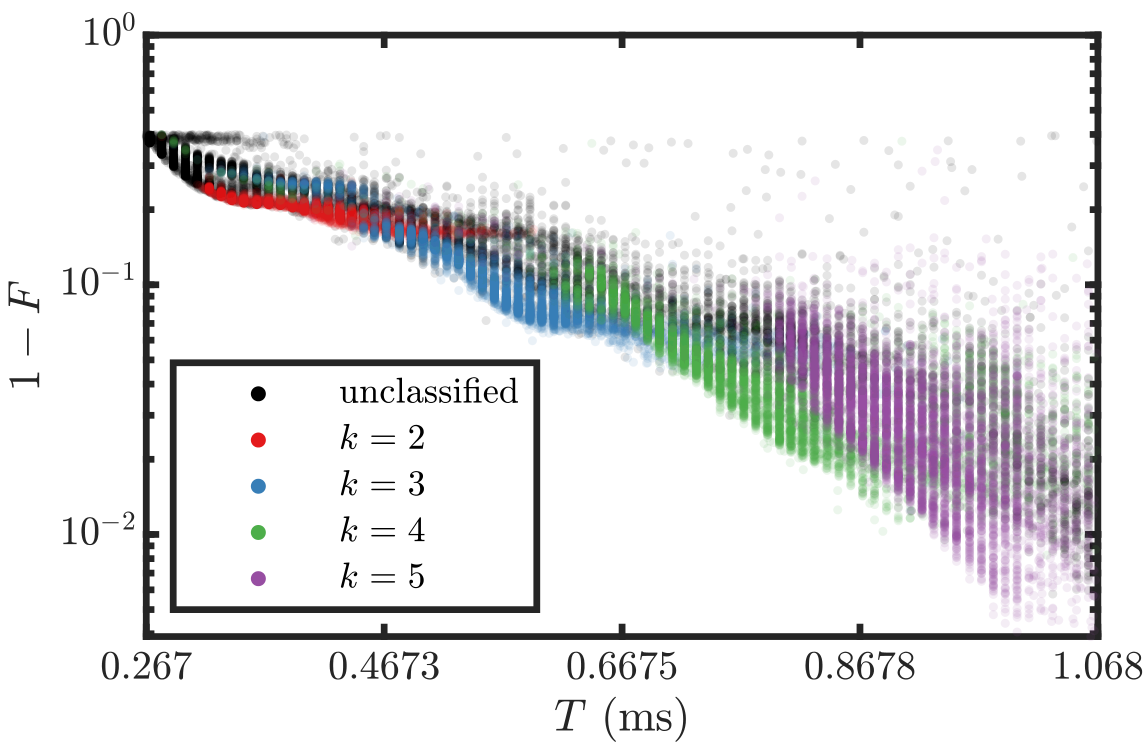
\includegraphics[width=\columnwidth]{graphics/clustering/QM2Screenshot.png}
	\end{subfigure}
	\begin{subfigure}{\columnwidth}
		\centering
		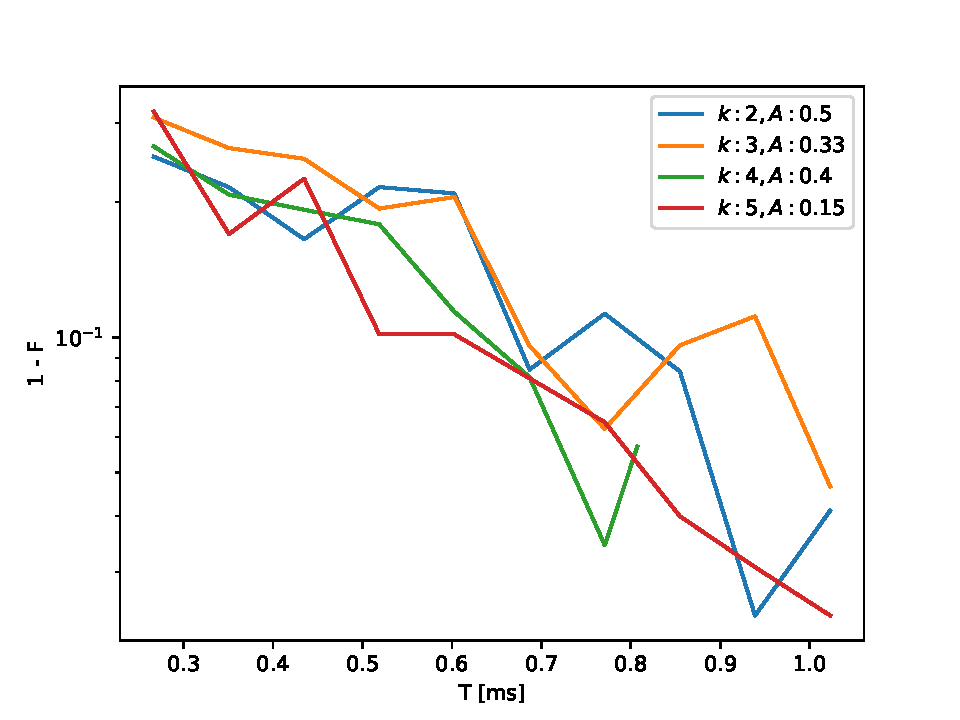
\includegraphics[width=\columnwidth]{graphics/clustering/QM2Clustering.pdf}
	\end{subfigure}
	\caption{
		\textbf{Upper}: This figure is taken from \cite{QM2Paper} and shows how optimized controls can be clustered by their projection onto $\cos(k\pi t/T)$. \textbf{Lower}: Infidelity of \proc{Grape} optimized solutions with initial control $u(t)=A\cos(k\pi t/T)$. The first axis shows the control duration $T$.}
	\label{fig:Clustering}
\end{figure}

As is also shown on the figure, seeds with different frequencies do not have the same amplitude. It was found that having a too high amplitude caused the state to become numerically unstable and the simulation to not function correctly as described in Sec. \ref{subsubsec:spatial-limitations-of-controls}. This is also the reason that the $k=4$ data spans a smaller time interval due to numerical errors in their solutions for $T>0.8 ms$. \\

% How can this be clustered in a simple way?
While it is currently not possible to calculate each feature $c_k$ with composer since the control functions cannot be extracted, it is still possible to analyze the screenshots of the controls. One way of classifying the controls using the screenshots is to count the number of 0-crossings the control performs. Since cosine functions of increasing frequencies perform an increasing number of 0-crossings, we would expect that optimized controls perform a number of 0-crossings proportional to the control duration. An example of this clustering method is shown in Fig. \ref{fig:SimilarTimescales} where two similar seeds are compared and the optimized control with highest duration has more 0-crossings.

\begin{figure}
	\begin{subfigure}{0.4\columnwidth}
		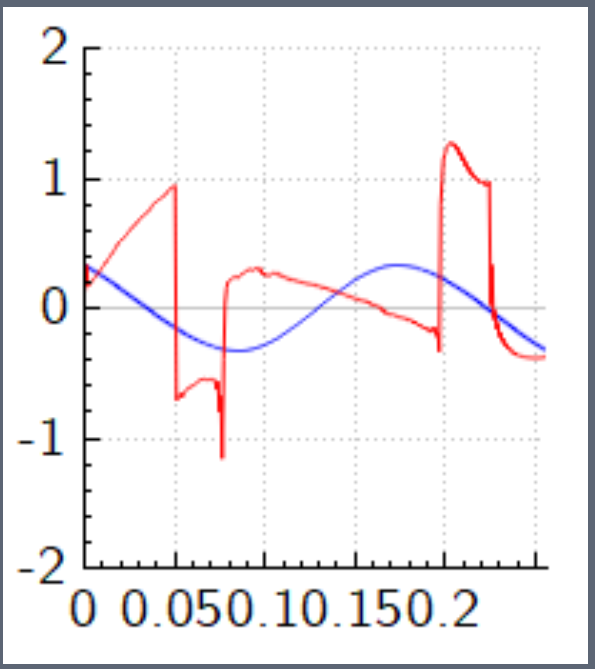
\includegraphics[width=\columnwidth]{graphics/similar_solutions/T02563k3A033.PNG}
	\end{subfigure}
	\begin{subfigure}{0.4\columnwidth}
		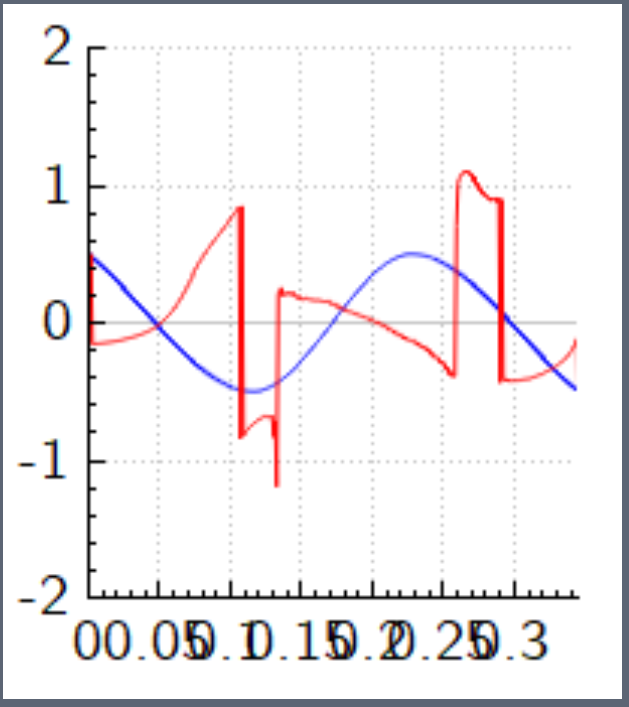
\includegraphics[width=\columnwidth]{graphics/similar_solutions/T03450k3A050.PNG}
	\end{subfigure}
	\caption{Screenshots of optimized controls of a similar seed ($k=3$) for 2 different durations and amplitudes. The axes show control displacement $u(t)$ as a function of time. \textbf{Left:} $T\approx 0.35$ms, $A=0.33$. \textbf{Right:} $T\approx 0.47$ms, $A=0.50$. The optimized seeds are very similar in terms of shape, but differ in the number of 0-crossings, where the left control has 5 and the right has 7.}
	\label{fig:SimilarTimescales}
\end{figure}

%Actually doing the clustering
All optimized solutions shown in Fig. \ref{fig:Clustering} were analyzed as well as some not shown results for the parameters $k=3$, $A=0.5$. Some data was not included as the optimized control screenshots were not saved. The results of counting the number of 0-crossings for each control are shown in Fig. \ref{fig:crossingsClustering}. The results seem to indicate that as the control duration is increased, so is the number of 0-crossings of the best performing solutions.  

\begin{figure}
	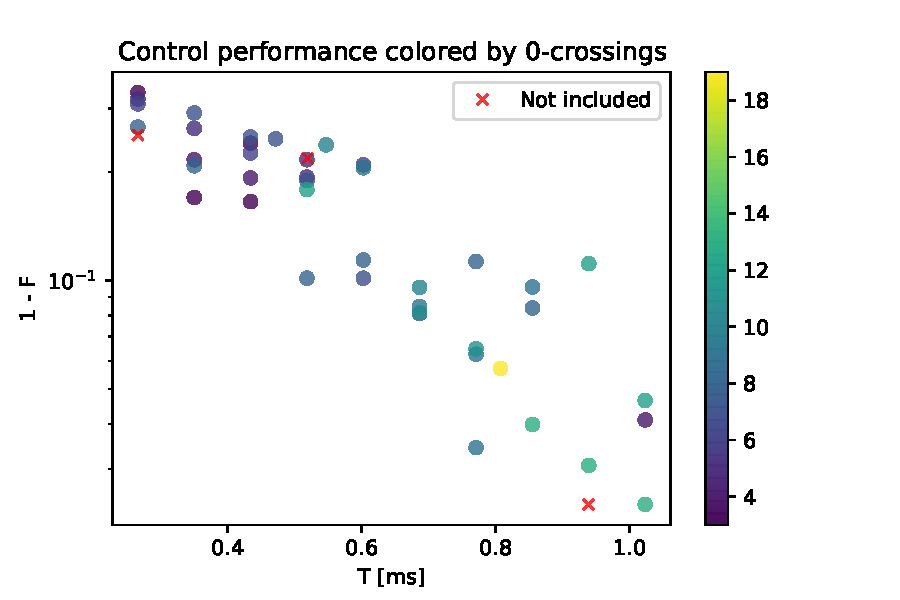
\includegraphics[width=\columnwidth]{graphics/clustering/crossings.pdf}
	\caption{The performance of the optimized controls from Fig. \ref{fig:Clustering}, colored by the number of 0-crossings. The analysis indicates that the number of 0-crossings in optimal controls increases with the control duration.}
	\label{fig:crossingsClustering}
\end{figure}


\subsection{Robustness of solutions} \label{subsec:robustness} 
The robustness of optimized solutions with respect to self interaction strength or potential scaling was studied in an article \cite{GroupPaper}. This is interesting since real experiments are often subject to the inherent uncertainties of their equipment e.g. the frequency width of a laser. Since the self interaction in a BEC is dependent on the number of atoms it consists of, it is not surprising that a specific strength $\beta$ is difficult to replicate exactly in the lab and may at the same time vary in time. Likewise the trapping potential is created by standing waves of laser light and so it is also subject to some uncertainty in intensity and frequency.  \\

The robustness of optimized solutions was explored for the system \textit{Composer implementation of Quantum Moves 2} described in Appendix \ref{App:System-params}. This replication was done by letting \proc{Grape} optimize the same control seed, $u(t)=0.15\cos(5\pi t/T)$, for $300$ iterations and for different durations $T=0.5$, $T=0.875$ or $T=1.3$, noting that these durations are respectively below, near and above the QSL of this system. These optimized solutions were then replayed in a system with a modified interaction strength $\tilde{\beta} = a_I \beta$ or in a system with a modified potential $\tilde{V}(x,u(t)) = a_V V(x,u(t))$.

The results can be seen in Fig. \ref{fig:robustness}. There seems to be an overall trend where the more optimal a solution is, the more sensitive it is to small changes in either the potential or the interaction, in terms of fractional change from the unperturbed case. Keeping in mind that better solutions are reached for longer durations, this could also be intepreted as how the 'fidelity landscape' becomes increasingly more complex the longer the control duration is. This could make sense since for small durations below the QSL, there could be many 'plateaus' near optimal fidelity. Small changes to the system would change the shape/height of the plateau, but if the changes are small then the optimized solution should still be somewhere on this plateau. On the contrary, for long durations above the QSL, the landscape is more ``spiked'' due to some specific solutions being able to reach very high fidelities and this spiked landscape would of course be more affected of changing parameters. \\

\begin{figure}
	\begin{subfigure}{\columnwidth}
		\centering
		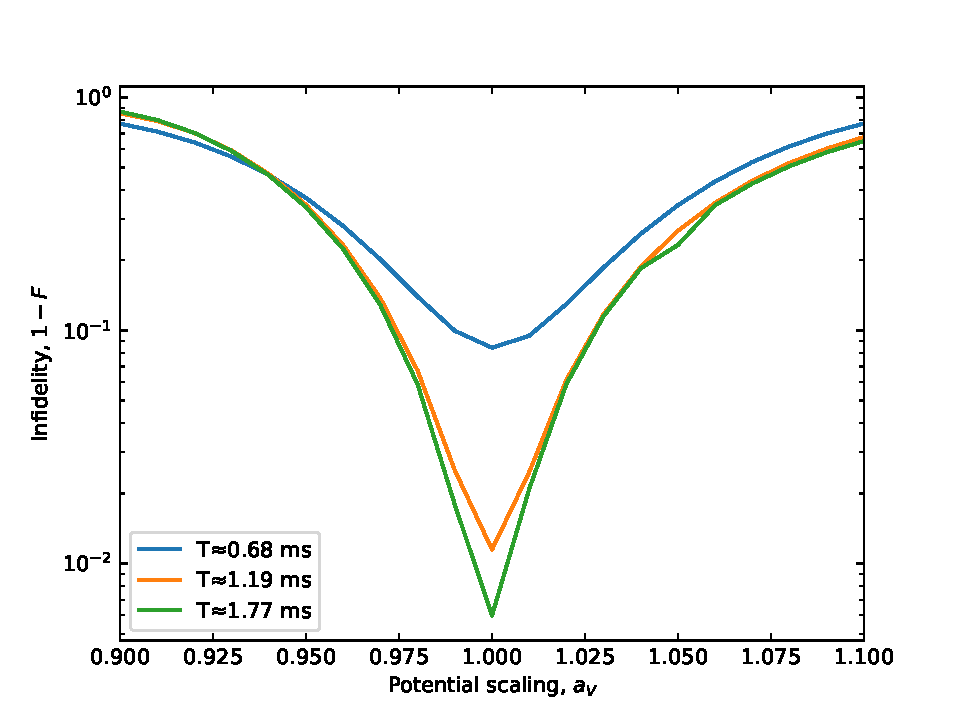
\includegraphics[width=\columnwidth]{graphics/robustness/robustness.pdf}
	\end{subfigure}
	\begin{subfigure}{\columnwidth}
		\centering
		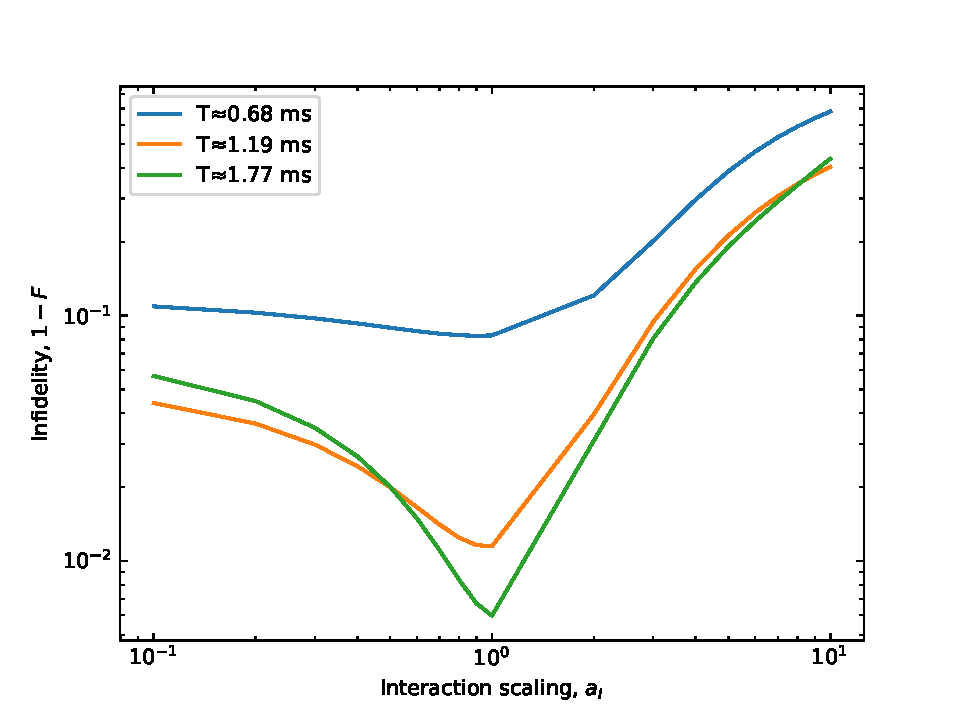
\includegraphics[width=\columnwidth]{graphics/robustness/interactionRobustness.pdf}
	\end{subfigure}
	\caption{Examining the robustness of an optimized solution. \textbf{Top:} By scaling the potential. \textbf{Bottom:} By scaling the BEC self interaction. The three control durations are chosen to be below, near and above the QSL of this system. The higher the control duration, the more relatively sensitive the optimized control is to noise.}
	\label{fig:robustness}
\end{figure}


\section{Strategies}\label{sec:strats}
%TODO Nævn evt noget om seeding strategy hvis det der står ikke er godt nok
%TODO Nævn et sted heri, at man i sin seeding strategy kan vælge enten at lave et kvalificeret gæt som er 'svært' at afvige fra (vilde bevægelser) eller et kvalificeret gæt som er vagt og derigennem kan man lade optimizeren føre det i den retning som er bedst. Her kan man evt. vise hvad der menes med et par figurer, hvor det ene seed er tæt på optimal løsning og det andet er ganske langt fra.
% Function vs graph approach
Throughout working with this project, there has been two ways to determine the control function $u(t)$ in Composer: The control function is determined either by an analytical expression (using the Scalar expression node) or it is made by dragging the desired ``path'' of displacement on a graph (using the Control node). These different nodes are shown in Fig. \ref{fig:Controls}. One can use both of these approaches when working with quantum control and they both have their advantages and disadvantages. \\

\begin{figure}[h]
	\begin{subfigure}[b]{0.4\columnwidth}
		\centering
		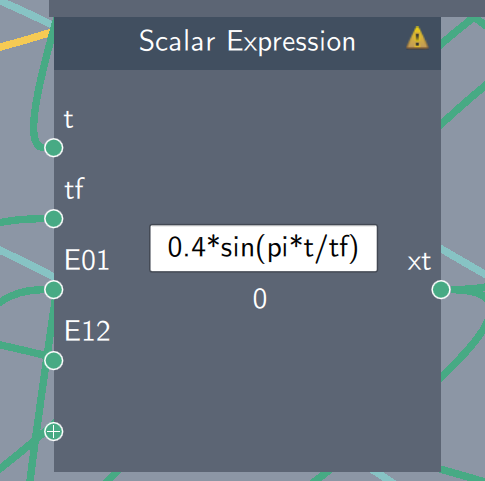
\includegraphics[width=\columnwidth]{graphics/composerScreens/ScalarExpressionNode.png}
		\caption{Scalar expression node}
	\end{subfigure}
	\hfill
	\begin{subfigure}[b]{0.45\columnwidth}
		\centering
		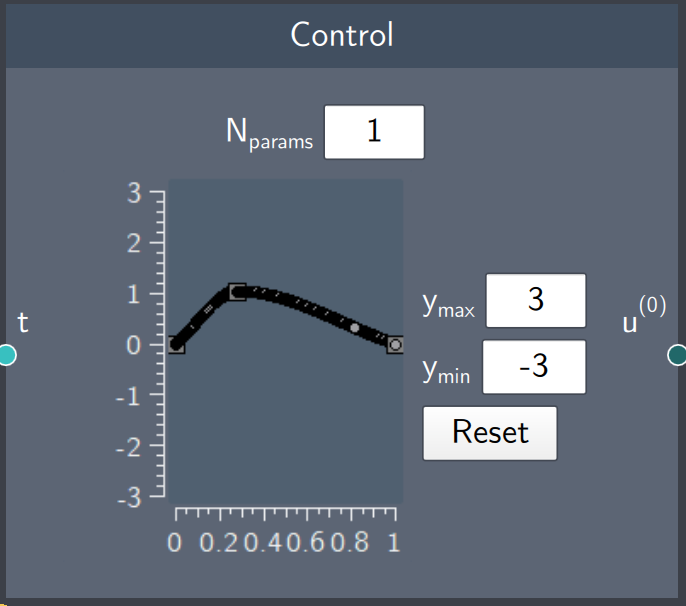
\includegraphics[width=\columnwidth]{graphics/composerScreens/ControlNode.png}
		\caption{Control graph node}
	\end{subfigure}
	\caption{Both nodes used for making a control function in Quantum Composer. The analytical function method (a) can take a number of input constants like final time $tf = T$, energy spacing between different states $(E01 = E_1 - E_0)$ and variables such as time $t$. The graph method (b) always scales the first axis such that the first point on the graph is at $t=t_0$ and the final point is at $t=T$.}
	\label{fig:Controls}
\end{figure}

% About function approach
Using an analytical expression as a control function, one gets the possibility of tweaking initial parameters to great accuracy such that the seed $\proc{Grape}$ gets already has a high fidelity. It is preferable to the graph approach in cases where a desired oscillation frequency is wanted e.g. the function $A\sin(E_{01}t)$. These kind of functions are difficult to mimic in the graph approach. When working with expressions independent of the final time $T$, adjusting this parameter translates into cutting the graph at different times. This is useful when exploring different functions and one finds that higher fidelity occurs at a different time than one currently works with. This method is shown in Fig. \ref{fig:funcAppr}. \\
\begin{figure}
	\def\svgwidth{\columnwidth}
	\input{graphics/strategies/functionAppr.pdf_tex}
	\caption{How an analytical control function can be used to reach a higher fidelity seed by altering the final time $T$. In this example we use the control function shown in red and the final time $T_1$. Evolving the system for a shorter (longer) time can yield a higher fidelity, and we can reach these fidelities by replacing the final time with $T_2$ ($T_3$). This method only works if the control function is independent of the final time.}
	\label{fig:funcAppr}
\end{figure}

% About graph approach
The Control graph node makes it possible to build up the control function as a series of steps. Here one can move one point on the graph and watch how the state evolves until that point, making it possible to optimize each step before going further. Since the graph node always spans the entire time interval $\{t_0,T\}$, this makes using the node useful when wanting to stretch or contract the entire function as shown in Fig. \ref{fig:graphAppr}. As demonstrated with the BEC in a harmonic potential in Fig. \ref{fig:HO}, there exists a complex relationship between $\beta$ and $T$ and so being able to keep the shape of the control function the same while altering the total time makes the node a beneficial tool to use.\\

\begin{figure}
	\def\svgwidth{\columnwidth}
	\input{graphics/strategies/graphAppr.pdf_tex}
	\caption{One method to optimize fidelity with the graph node. Changing the control time $T$ will squeeze or stretch the control function. Altering the final time can be beneficial given the complex relationship between $\beta$ and $T$, but also as a tool to regulate the speed at which the potential moves. Using this approach also allows us to fix the control end points, e.g. $u(0)=u(T)=0$ for any $T$. This should be compared to the analytical function approach shown in Fig. \ref{fig:funcAppr} where this is not always the case and the state could possibly need to be transported back to its initial position.}
	\label{fig:graphAppr}
\end{figure}

When calculating the maximum reachable fidelity for some combination of $\beta$ and $T$ in the harmonic potential, the graph control node was used to seed the $\proc{Grape}$ algorithm. The overall strategy using this tool involved moving points on the graph into certain shapes and looking at how the initial (i.e. no $\proc{Grape}$) fidelity looked. I particularly liked the semi-circle shape of a $\sin(\pi t/T)$ function where the amplitude was varied. Another particular shape used in this work was generated by moving a single point around $0.1T$ or $0.9T$ to create a function which had a fast(slow) buildup to a maximum and then a slow(fast) return to the initial position. This wedge-like shape is shown in Fig. \ref{fig:Controls} (b).

Both of these strategies worked well and provided nice seeds for $\proc{Grape}$ to optimize on. Despite some cases where the fidelity changes significantly from small variations of $\beta$, the overall rule seems to be that something that works well for one value of $\beta$ will have a similar fidelity for nearby values of $\beta$, and so this was also used to find a good seed when $\beta$ was larger than $10$, since above this limit the system seemed a lot more sensitive to the initial control function with respect to reaching the highest possible fidelity for that particular combination of $\beta$ and $T$. \\

Measuring the Quantum Speed Limit for the quartic system (\textit{B1} in Appendix \ref{App:System-params}) involved a combination of 2 strategies: The self-dubbed "up-to-down" and "down-to-up" approaches. \\

\proc{Up-to-down}:
\begin{enumerate}
	\item Pick $T_{up}$ to be a control duration estimated to lie above the QSL of the system
	\item Find an optimizable solution capable of reaching $F~0.99$
	\begin{itemize}
		\item If unable to do so, return to Step 1 and choose a higher $T_{up}$
	\end{itemize}
	\item Gradually lower the duration in small steps, ensuring at each step that the control can still be optimized to $F~0.99$
	\begin{itemize}
		\item If the control is unable to reach $F~0.99$, one should try minor modifications to the control to see if this fixes it. This could be dragging a point on the control graph slightly up / down to increase fidelity.
	\end{itemize}
	\item The lowest reachable $T$ is then the estimate of the QSL for the system. These steps can be repeated for another control function.
\end{enumerate}
The \proc{Up-to-down} procedure was my main method for estimating the QSL of the system shown in Fig. \ref{fig:QSL}.\\

\proc{Down-to-up} works in a similar way to \proc{Up-to-down}, but in a reversed way.
\begin{enumerate}
	\item Pick $T_{down}$ such that it is estimated to lie below the QSL of the system.
	\item Try a number of different control functions and choose the most promising (i.e. the seed capable of reaching highest fidelity)
	\item $T$ is raised in small steps, at each step optimized and modified to check if $F~0.99$ is reachable
	\item The first time $F~0.99$ is reachable, the current $T$ is the estimated QSL for the system.
\end{enumerate}
This procedure attempts to exploit that the optimization landscape for \proc{Grape} to traverse is hopefully simpler due to the lower control duration that is then gradually raised in the hopes that the seed has found a potential fidelity peak in the landscape that becomes available for some slightly higher control duration.

%Cos vs Sin funcs
While reproducing the clustering of optimized controls data seen in Fig. \ref{fig:Clustering}, it became apparent that using cosine functions instead of sine functions could be advantageous for small timescales. One can use the fact that cosine is displaced from 0 at $t=0$ to one's advantage as it initially places the state on a steep slope of the potential. This generates motion of the state much faster than when initiating with a non-displaced control function. Similarly when the control is done, one can displace the potential such that the state feels rapid deceleration, thus reducing the velocity of the state much faster than if the control was constrained to end at $u(T)=0$. This behavior can also be seen on the optimized controls shown in Fig. \ref{fig:similarSolutions}, where both end points experience rapid displacement away from $x=0$. These advantages are similar to the "back-swing" solution for another quantum control problem described in \cite{QM2Paper}.

\section{QEngine}\label{sec:QEngine}
This section describes the work done using the QEngine, a C++ library which Quantum Composer is build on top of \cite{ahmed2020quantum, QEngine}. Instead of the GUI that Composer offers, it is library of efficient methods for simulating quantum mechanics. This makes it vastly more flexible and customizable than the graphical interface built onto it. The QEngine library comes with a number of example files that can be modified to set up a desired system and e.g. a control function with optimization using one (or all) of the three available optimizers. The \texttt{DataContainer} class can be assigned to save variables, control functions, etc. and can be saved in either \texttt{.mat} or \texttt{.json} format to later be read by either \proc{Matlab} or anything else, respectively. Similarly to the Composer case, the data gathered using the QEngine is further analyzed and plotted using \proc{Python}. \\

% Unoptimized simulation / Comparison
To start off an exploration into the advantages that QEngine offers compared to Quantum Composer, a previously examined problem is replicated using the QEngine. The replicated problem is the periodically shaken potential shown in Fig. \ref{fig:beta} and the QEngine results are included in Fig. \ref{fig:QEngine_nonOPt}. The two tools reach the same or very similar fidelities for simulations where $\beta > -13$. Below this limit, the results follow the same trend, but it appears that the system becomes very sensitive to the final time.
\begin{figure}
	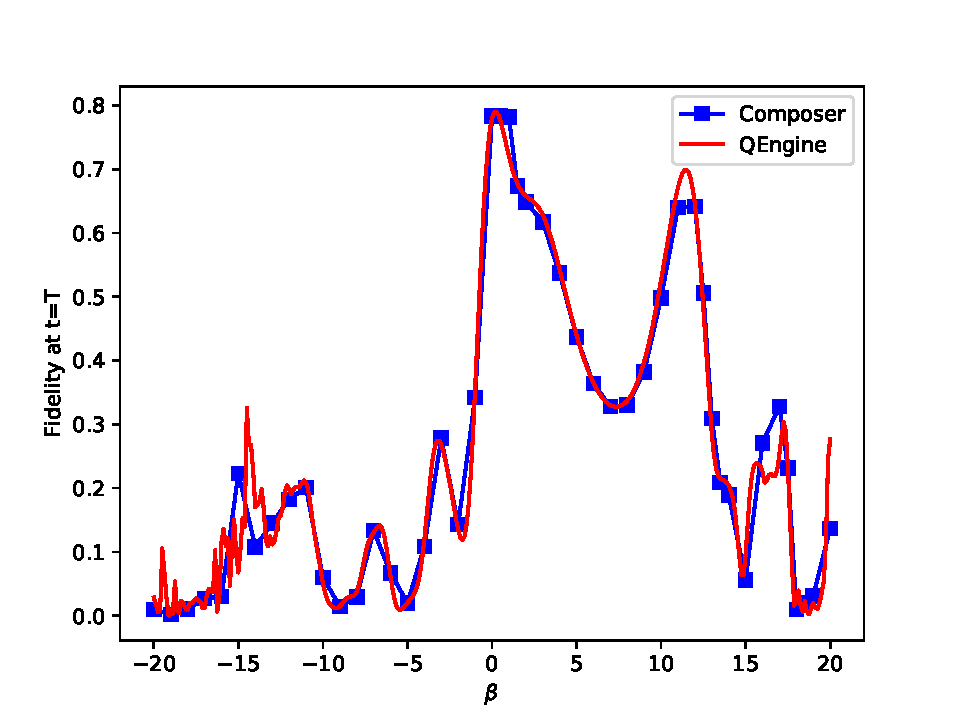
\includegraphics[width=\columnwidth]{graphics/qengine/comparison.pdf}
	\caption{Comparison of the results obtained using Composer and the QEngine where both tools simulate the unoptimized control from Eq. \eqref{eq:nonopt-control} with a control duration of $T=3.49$. The two tools reach the same or very similar results for most of the self interaction values, which is also expected as Quantum Composer uses the QEngine for computations. The parts where the 2 tools disagree are suspected to be caused by numerical inaccuracies.}
	\label{fig:QEngine_nonOPt}
\end{figure}

% Clustering of QEngine results
\subsection{Clustering of controls}\label{subsec:qengine-clustering}
In the following it is demonstrated how the QEngine exceeds Quantum Composer as a data gathering tool. The system is set up in the exact same manner as the system described in Sec. \ref{subsec:composer-clustering}. A seed is set using an analytical expression. From this initial seed, a number of new seeds $n$ are generated by adding random noise to each point of the discretized control. Each of these noisy seeds are optimized, some using only \proc{Grape}, others with \proc{Group} and d\proc{Group} as well. 

The resulting infidelity of these optimized solutions are shown in Fig. \ref{fig:QEngine_noise}, where the best results from Composer in Fig. \ref{fig:Clustering} have been included for reference. From each initial seed with added noise, it is possible to calculate many more datapoints and optimize seeds to reach higher fidelities than what is possible in Composer, even when \proc{Grape} does the optimization. This is most likely a result of having a high iteration cap $N_{max}=3000$ on the optimizer in the QEngine. This out performance of Composer does come at the cost of a considerable computation time, though. The exact settings and seeds used are listed in Appendix \ref{App:QEngine-settings}.

\begin{figure}
	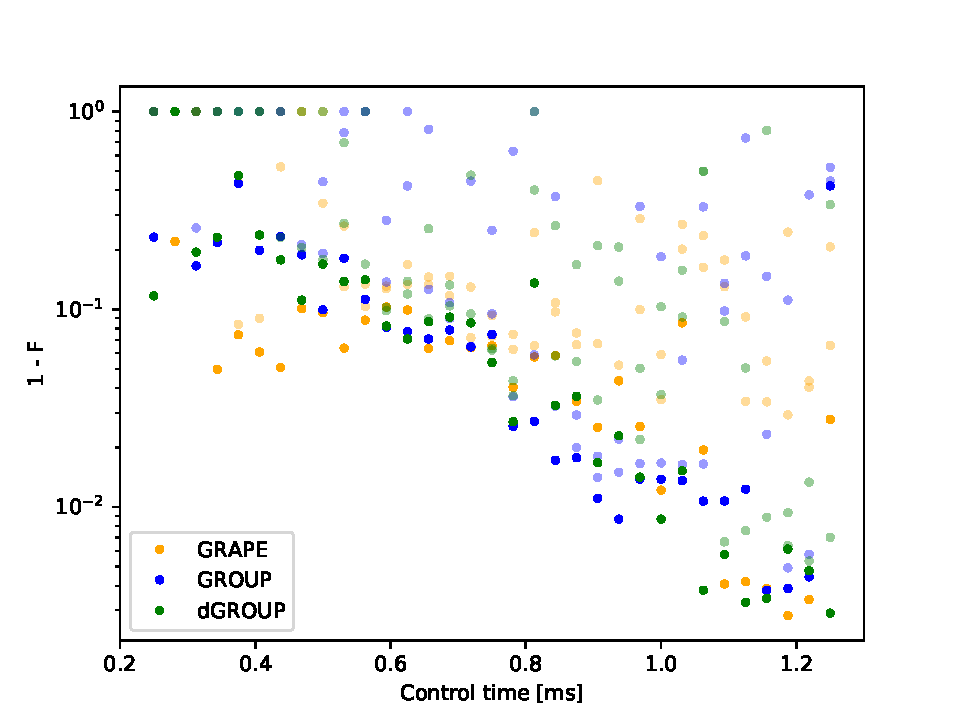
\includegraphics[width=1.1\columnwidth]{graphics/qengine/noiseDemoInf.pdf}
	\caption{Infidelities of solutions optimized using each of the 3 optimizers available in the QEngine: \proc{Grape} (yellow), \proc{Group} (blue) and d\proc{Group} (green). }
	\label{fig:QEngine_noise}
\end{figure}

It was not possible to replicate the clustering of optimized controls similarly to what was done in Ref. \cite{QM2Paper} using Quantum Composer as mentioned in Sec. \ref{subsec:composer-clustering}. This is, on the other hand, possible using the QEngine, where optimized controls and expectation values are extracted using the \texttt{DataContainer} class.

The optimized controls shown in Fig. \ref{fig:QEngine_noise} were chosen if $\mathcal{F}[u] \geq 0.70$ and clustered by calculating a vector of features $\vec{c} = (c_0, \dots, c_5)$ using Eq. \eqref{eq:QM2-ck-expression}. The feature vectors were clustered using the \proc{dbscan} method from the \texttt{sklearn} Python module with parameters $\epsilon = 0.05 $, 
$\min_{\text{samples}} = 10$ and Euclidean metric. This is the same clustering method using in Ref. \cite{QM2Paper}. \proc{dbscan} works by finding \textit{core samples} defined as containing $\min_{\text{samples}}$ other points withing a distance of $\epsilon$ of them in feature space. A collection of these core samples are then considered a cluster. The results of the clustering are shown in Fig. \ref{fig:QEngineClustering}.

\begin{figure}
	\begin{subfigure}{\columnwidth}
		\centering
		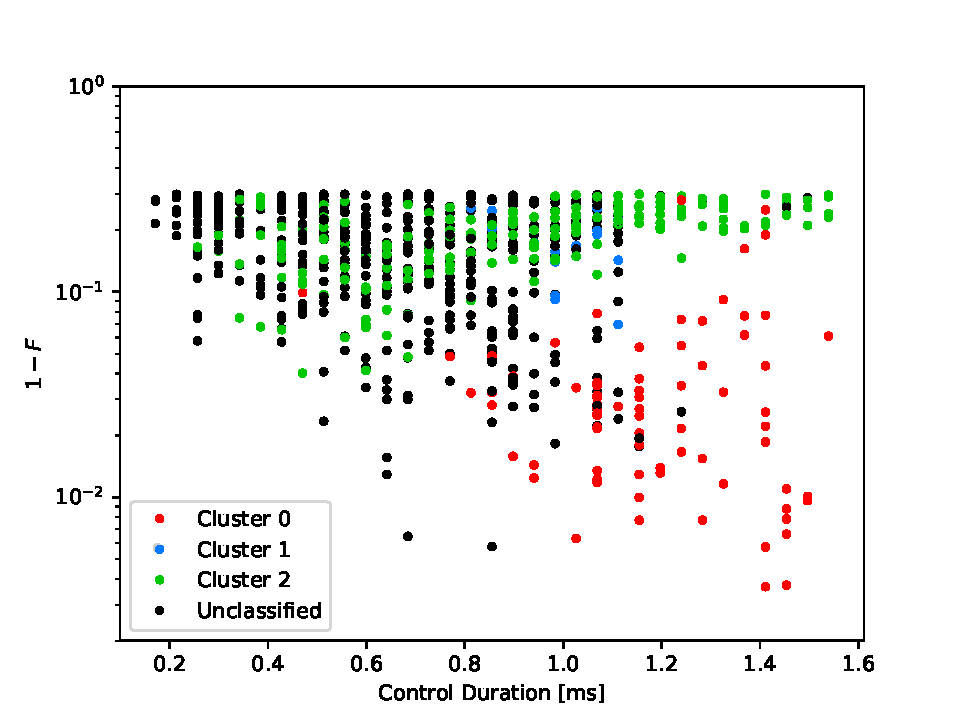
\includegraphics[width=\columnwidth]{graphics/qengine/QEclustering-classification.pdf}
	\end{subfigure}
	\begin{subfigure}{\columnwidth}
		\centering
		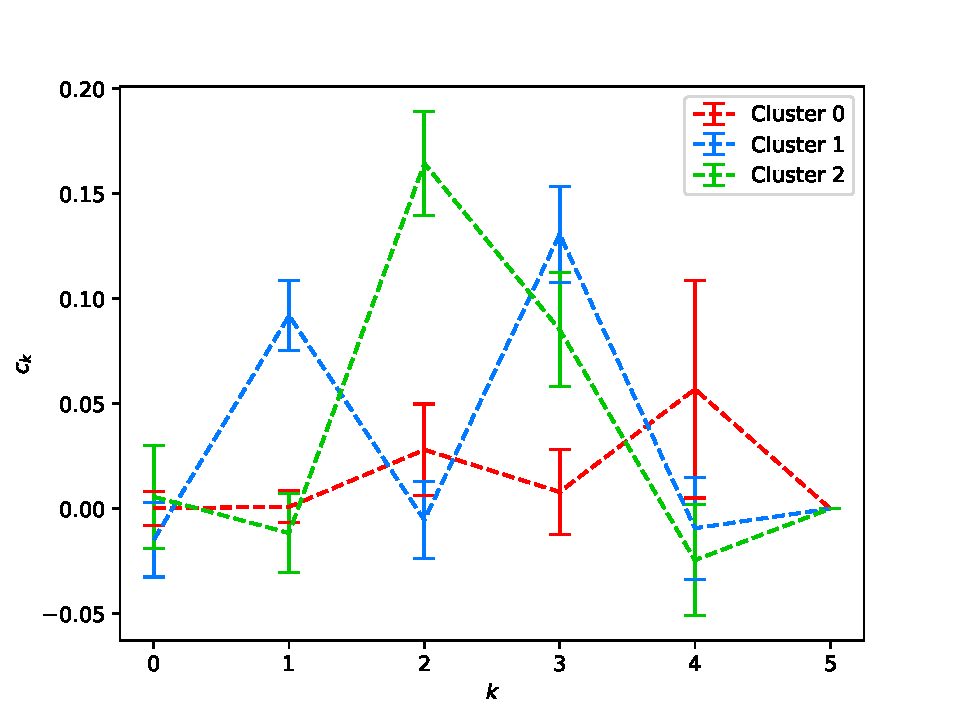
\includegraphics[width=\columnwidth]{graphics/qengine/QEclustering-features.pdf}
	\end{subfigure}
	\begin{subfigure}{\columnwidth}
		\centering
		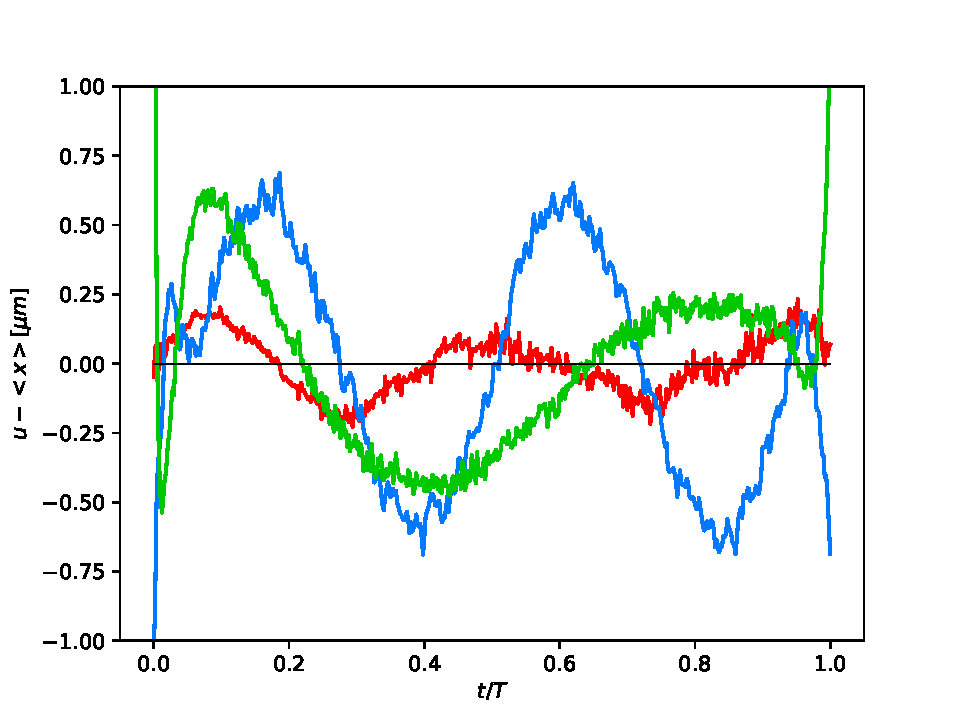
\includegraphics[width=\columnwidth]{graphics/qengine/QEclustering-means.pdf}
	\end{subfigure}
	\caption{Clustering of the data presented in Fig. \ref{fig:QEngine_noise} in a similar way to what was done in Ref. \cite{QM2Paper}, seen at the top of Fig. \ref{fig:Clustering}. \textbf{Top:} Time vs. infidelity plot showing which points belong to which clusters. Black points have not been assigned a cluster. \textbf{Middle:} Mean feature vectors of each cluster. Errorbars show the standard deviation. \textbf{Bottom:} Average motion of $u(t)-\langle x(t) \rangle$ for each cluster. The thin black line marks $u(t)=\langle x(t) \rangle$ for visual aid purposes. Note that cluster $2$ (green) begins and ends at values above \SI{1}{\micro\meter}.}
	\label{fig:QEngineClustering}
\end{figure}

Based on the results shown, we can conclude a number of things. Firstly it is clear that the clusters found are not concentrated around the lowest infidelity regions, but instead span a large duration and infidelity interval. In order for the algorithm to find clusters in the optimal time-infidelity regions, a much higher density of data points are needed as seen in the original figure from Ref. \cite{QM2Paper}. 

If we focus on the clusters that have been found, we see that cluster mean feature vectors have identified clusters dominated by different cosine frequencies. From these clusters we see that Cluster 0, mainly consisting of controls in the upper half of the durations simulated, is dominated by the highest cosine frequencies. Thus, we find the same trend as described in Ref. \cite{QM2Paper} where the optimal solutions at higher durations could be characterized by a higher frequency.

Considering the relative controls $u(t) - \langle x(t) \rangle$ that emerge, we see that Cluster 1 and 2 (blue and green on the figure) behave similarly. They both begin with $u(t)\neq 0$ and oscillate with a higher relative amplitude than Cluster 0, which is not displaced at $t=0$ and generally has a lower relative amplitude. 

\subsection{Landscape exploration} \label{subsec:qengine-landscape-expl}
In a recent group meeting presentation \cite{MogensQMMG} it was attempted to describe the control landscape of a 1D chain of 5 spin-$1/2$ particles. This was done by calculating a number of characteristics based on many optimization runs: Infidelity, mean step size, no. of unique optimized controls and the mean of the Hessian diagonal. Infidelity offers insight into the height of the landscape and the number of local ``traps'' in that part of the region. A trap is a local maximum named so since it can ``trap'' a gradient based optimizer and keep it from reaching the global maximum. The mean step size could hopefully describe how ``flat'' the landscape is, i.e. a large (in this case around unit length) step size means that we get a similar fidelity score from a control that is similar to the current one. The number of unique controls show the number of different solutions that are found in that simulation. The Hessian diagonal describes tries to describe how sharp the found peaks are in the control space.


A control $u(t)$ is in this case different from another control $v(t)$ if the Euclidean norm between the two controls is larger than $\epsilon$
\begin{equation}
	u \text{ different from } v \Leftrightarrow \left(\sum\limits_{i} [ u(t_i) - v(t_i) ]^2 \right)^{1/2} > \epsilon
\end{equation}
with $\epsilon = 10^{-16}$.

The Hessian diagonal is calculated numerically using finite differences \cite{fornberg1988generation}, which states that given a grid with uniform spacing $h$, the second derivative of a function $f$ at a point $x$ can be approximated to second order in accuracy by 
\begin{equation}
	f''(x) \approx \frac{f(x+h) - 2f(x) + f(x-h)}{h^2}.
	\label{eq:qengine-landscape-finite-differences}
\end{equation}

In practice the Hessian diagonal was approximated using the following procedure.
\begin{enumerate}
	\item Extract optimized control $\vec{u}$ and fidelity $\mathcal{F}(\vec{u})$.
	\item For each timestep in $\vec{u}$:
	\begin{enumerate}
		\item Obtain $\mathcal{F}(\vec{v}^{(i)}_\pm)$ with $\vec{v}^{(i)}_\pm = (u_0, \dots, u_i \pm h, \dots u_N)$ by simulating the control.
		\item Approximate the second partial derivative $\frac{\partial^2}{\partial u_i^2} \mathcal{F}(\vec{u})$ using Eq. \eqref{eq:qengine-landscape-finite-differences}.
	\end{enumerate}
\end{enumerate}

The QEngine was set up to run 25 iterations for each final duration. The \proc{Grape} optimizer was set up with parameters $N=1000$, $\gamma = 10^{-5}$ and boundaries $u(t) \in \pm \SI{2}{\micro\meter}$ with weight $\sigma = \num{2e3}$. In an attempt to search a larger part of the control space, the seeding strategy consisted of using cosine and sine functions with randomized amplitudes and frequencies described in the following equation

\begin{equation}
	u_{landscape} = A \cos(k_1 \pi t/T) + B\sin(k_2 \pi t/T)
	\label{eq:qengine-landscape-seed}
\end{equation}
with $A,B \in \{-0.5,0.5\}$ and $k_1,k_2 \in \{-3,3\}$ being randomly generated for each control.

The resulting controls with $\mathcal{F}(u) \geq 0.1$ were kept for further analysis and the rest discarded. The quantities of interest mentioned above were calculated based on the remaining controls. These have been plotted on Fig. \ref{fig:qengine-landscape}. Most of the quantities calculated are not easily interpreted. The mean step size gradually decreases as control duration increases. Could indicate that the control landscape becomes more ``rugged'' as time increases as described previously. Despite the attempt to thoroughly explore the control landscape using the seeding strategy in Eq. \eqref{eq:qengine-landscape-seed} it could be interesting to see how much the results would change from the inclusion of a new set of data. 

\begin{figure}
	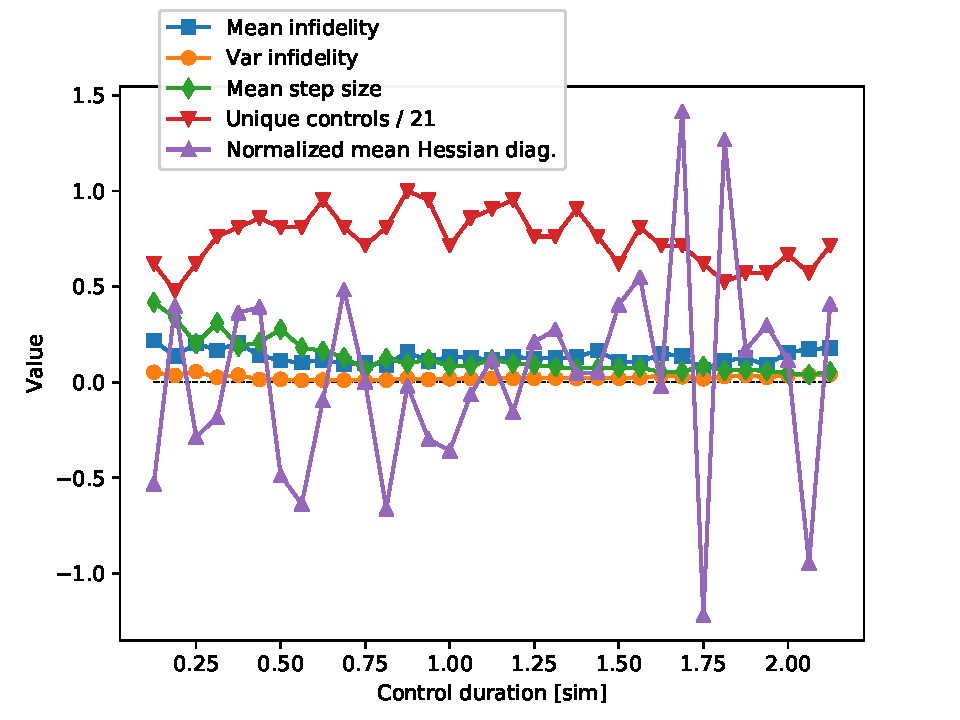
\includegraphics[width=\columnwidth]{graphics/qengine/landscapes/Landscape.pdf}
	\caption{Calculated quantities of interest for describing the control landscape. The gradual decrease in mean step size as control duration $T$ is increased could indicate that the number of local traps increase with duration. The mean Hessian diagonal was expected to be negative for all times since this would indicate a fidelity ``hill''. Instead it fluctuates between positive and negative values and even for nearby durations there is a big difference. }
	\label{fig:qengine-landscape}
\end{figure}

\subsection{Seeding strategies}\label{subsec:qengine-seeding-strats}
%TODO This section should contain some of my thought for generating seeds that exhaust ctrl. space
%TODO Seeding strat cant be completely simple, because of the way seeds looked in QM2 shakeup, this could serve as a method for generating seeds in composer
This subsection will attempt to expand upon the lack of ``control landscape'' exploration mentioned in Sec. \ref{subsec:qengine-landscape-expl}. The goal will be to formulate a strategy that is able to ``globally'' point to a region in the control space that can then be locally explored using pseudo-randomly generated numbers for the specific controls.

The seeding strategy $U$ is computed in the following way
\begin{equation}
	U = S \times A (T_s - D)
	\label{eq:seeding-strategy-formalism}
\end{equation}
where $S$ is a scaling factor that can be used to bound controls within an interval of values, $A$ is the amplification strategy, which will amplify a certain region of the control e.g. points near the halfway point, $T_s$ is the \textit{term strategy} which denotes the number of and type of terms the control consists of. This could for instance be 4 cosine terms of increasing frequency $\sum_k \cos(k \pi t/T)$. Finally $D$ is the \textit{displacement} which can be used to ensure certain boundary conditions such as $u(0)=u(T)=0$.

Once the strategy for calculating $U$ is in place, it is time to generate candidate strategies for further analysis. This was done by formulating sub strategies for each of the components in Eq. \eqref{eq:seeding-strategy-formalism} save for the scaling $S$, which was set to $1$ in all cases. These potential sub strategies are listed below.

\begin{itemize}
	\item[$A$] \textbf{- Amplification}
	\item \textit{Middle} - Scales the control around the midpoint $u(\frac{T}{2})$ by a factor of 3 with the $2\sin(\pi t/T) + 1$ while leaving endpoints the same.
	\item \textit{Endpoints} - Scales to control around the endpoints by a factor of 3 while leaving the middle untouched using $\cos(2 \pi t/T) + 2$.
\end{itemize}

%TODO Skriv om til matematisk udtryk i stedet?
\begin{itemize}
	\item[$T_s$] \textbf{- Term structure}
	\item \textit{Altcos} - \\ $\cos(r 2\pi t/T) + \sin(2r \pi t/T) + \cos(3 r 2\pi t/T) + \cdots$
	\item \textit{Altsin} - Similar to \textit{Altcos}. Alternates between sine and cosine terms starting with sine.
	\item \textit{Both} - $\sum_k \cos(2rk\pi t/T) + \sin(rk\pi t/T)$.
	\item \textit{Cos} - $\sum_k \cos(2rk\pi t/T)$.
	\item \textit{Sin} - $\sum_k \sin(rk\pi t/T)$
\end{itemize}

\begin{itemize}
	\item[$D$] \textbf{- Displacement strategy}
	\item \textit{Cosine} - Each term will be displaced to ensure the condition $u(0) = 0$.
	\item \textit{Frequency} - Instead of the frequency being $rk\pi t/T$ where $r\in[-1,1]$ is a randomly generated number, it will instead be set to $1$.
	\item \textit{Both} - Here both the cosine strategy and the frequency strategy will be used. This ensures the condition $u(0) = u(T) = 0$. 
\end{itemize}

Each combination of the above listed strategies had 25 of their controls plotted. After going through each strategy, 6 were chosen to be tested on the Quantum Moves 2 Shakeup problem. At each of the 9 control durations, 20 controls were generated using each strategy and optimized for up to $1000$ iterations using \proc{Grape}. Other optimization parameters used was $\gamma = \num{e-5}$ and $\sigma = \num{2e3}$ with boundaries $\pm\SI{2}{\micro\meter}$. These 6 were selected based on the controls resembling what could be made in Quantum Composer using the graph node described in Sec. \ref{sec:strats}. 

The chosen strategies are referred to in the form \textit{$T_s$-A-D-n} with $n$ being the number of terms. Their performance is plotted in Fig. \ref{fig:qengine-seeding-strats}, where both the best performing control and the first through third quartiles are shown for each strategy. Up to a control duration of \SI{0.75}{\ms} the strategies have similar performance and little spread. After passing \SI{1}{\ms} there is an increase in the spread of the strategy quartiles. The same thing is seen for the best controls. 

Note that no strategy using the \textit{sine} and \textit{altsin} term strategies were used. This is because these particular term strategies produced solutions that were all very similar to each other in terms of shape, unlike the other strategies.

\begin{figure}
	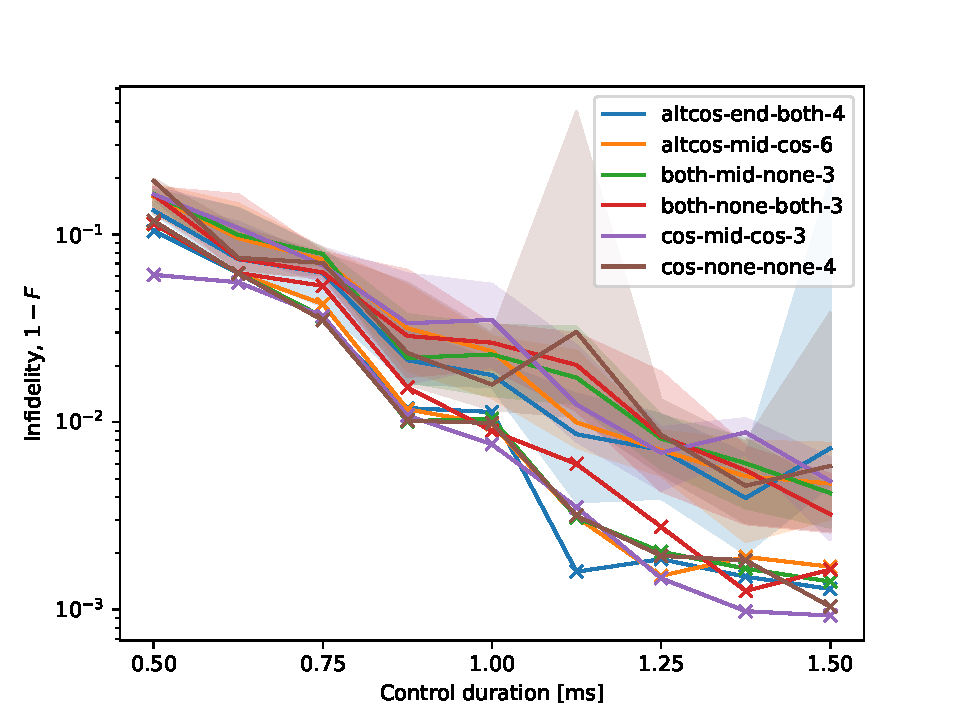
\includegraphics[width=\columnwidth]{graphics/strategies/seeding_strats_results/quantiles.pdf}
	\caption{Performance of 6 chosen strategies. The median (solid line) and upper/lower quantiles (shaded area) of the 20 controls for each strategy are drawn. The best solution for each strategy is marked by an X. 2 strategies stand out in a positive way. The first one is 'cos-mid-cos-3' found the best overall solution in 6 out of 9 control durations. The second one is 'altcos-end-both-4' which has the overall best performing median of the tested strategies.}
	\label{fig:qengine-seeding-strats}
\end{figure}

Overall it seems that this method of generating seeds can work as a way of exploring the fidelity landscape of the Shakeup problem. Comparing the found results to those obtained in Fig. \ref{fig:QEngine_noise}, we see that while the estimated QSL using these strategies is around \SI{0.85}{\ms} compared to around \SI{0.65}{\ms}, the solutions generated without the random noise seem to make up more ``optimizer-friendly'' seeds that are generally capable of reaching at least $\mathcal{F}\geq 0.8$ compared to those generated with random noise where many do not even reach this level. The strategies also keep up or outperform the optimized controls that were found in Composer, indicating that for anything but superficial exploration some kind of systematic seed generation method is necessary. This method could potentially be implemented in Composer as an expansion of the function node and with a new node generating random numbers. This would open up the possibility of doing much of the work that currently requires the QEngine (expert) tool instead of a simpler and more widely available tool.
%TODO Check up of whether the solutions generated here are more jittery like those from the clustering part.

\subsection{Optimal control analysis}
%TODO This section should be about the optimal controls that reach benchmark and an analysis of these

\section{Comparison}\label{sec:comparison}
As has been demonstrated, QEngine offers several advantages to Quantum Composer with respect to flexibility and computational power. However, this does not mean that the QEngine should be used for every problem. Quantum Composer makes it very easy to set up a desired system, run a simulation on that system and get the system plotted as the system evolves. This makes it preferable to use Composer when one wants to visually and (more or less) playfully explore the behavior of a system as the different parameters are tuned up or down.

Here, I will attempt to list some of the pros and cons of both tools.
\begin{itemize}
	\item[] \textbf{QEngine} 
	\item[\bf+] Flexible and customizable
	\item[\bf+] 3 Optimization algorithms
	\item[\bf+] Superior data gathering capabilities
	\item[\bf{--}] Data must be plotted seperately
	\item[\bf{--}] Data gathering can be \textit{very} time consuming
	\item[\bf{--}] Steep learning curve
	\item[\bf{--}] Difficult installation process
\end{itemize}

\begin{itemize}
	\item[] \textbf{Quantum Composer} 
	\item[\bf+] Many visualization options
	\item[\bf+] Intuitive to explore a given system
	\item[\bf+] Graph node to drag out a control function
	\item[\bf+] Simulating and optimizing is usually fast
	\item[\bf{--}] Limited flexibility and customization
	\item[\bf{--}] Most types of data must be manually gathered
	\item[\bf{--}] Some types of data cannot be exported from the program at all
\end{itemize}

Based on the considerations above it is concluded that Quantum Composer is preferable to use as an exploration tool. It is fast to set up, relatively easy to use and most importantly, it is very good at visualizing the simulation through its different kinds of plotting nodes. An example of this exploration could be a physicist trying to simulate an experiment to get a feeling for what kind of settings the experimental apparatus should be capable of. With the current state of Quantum Composer, I find it advantageous to use the QEngine for any kind of simulation where more than around 15 datapoints are desired. While the QEngine has a vastly steeper learning curve, it is designed to easily generate large amounts of data using computationally efficient calculations. It should also be mentioned that, in my personal opinion, having worked or used Composer before working with the QEngine might have smoothed the learning curve of using the QEngine. This is because many of the nodes in Composer correspond to a class in the QEngine library (remember that Quantum Composer is built on top of it) and so one can use the intuition of how the nodes are connected in Composer to find out how to set up a system in the QEngine. The example files provided with the library are also of great help to get started. These conclusions about when to use Quantum Composer align well with what the intended strengths of Composer are \cite{ahmed2020quantum}.\\

It could be advantageous to combine the playful, visual and fast elements that Composer has, with the more systematic, flexible and superior data gathering of the QEngine. One way to possible exploit the best of both these tools could be to use Quantum Composer for globally exploring a given system through the intuitive and playful graph control node. Any promising candidates for good seeds could be exported from Composer in the \texttt{.csv} format to be read by a QEngine script, where noise and other more local optimization approaches could be utilized.

These considerations also give rise to a number of suggestions for desirable features for Quantum Composer in order to make it more attractive to use as an expert tool. Most of these points are a result of a brainstorming/discussion session with Shaeema Ahmed (Aarhus University) and Tiantian Zhang (TU Vienna).

\begin{itemize}
	\item[] \textbf{Desirable features for Quantum Composer} 
	\item Conversion of real world data to dimensionless input scalars
	\item Exportable control functions to potentially be used in experiments
	\item Save data even when for-loops have run
	\item Import control functions from an experiment
	\item Enhance data gathering capabilities all around
	\item Select a time range for control durations
	\item Feed analytical control functions to \proc{Grape} optimizer
	\item Add noise to the control function
	\item A more detailed description of how to use the GPE spectrum node
	\item Undo and redo buttons
	\item An ability to automate data gathering, including exporting data
\end{itemize}

\section{Discussion}\label{sec:discussion}
As described in section \ref{subsec:numericalLimitations}, some of the ways to explore this problem are blocked by numerical instabilities. This could possibly be fixed by increasing the number of timesteps, which is currently $501$, since the smaller the timestep used, the better an approximation each step forwards in time becomes. This might mean that the GPE spectrum would have to be recalculated to minimize the variance of important states, but also mean an increased computational cost of each simulation.

%Composer Spectrum discussion
The energy spectrum is generated in Quantum Composer to create wave functions, find energy levels and calculate variances wrt. $\hat{H}_{GPE}$. This generation is subject to some initial guesses that can be tweaked to minimize the variance of any relevant states, thus ensuring that the simulation will be as accurate as possible. However, it seems to be the case that while one can tweak these guesses to reach low variances (on the order $10^{-8}$ or better) for one set of system parameters (e.g. $x_{max}$, $x_{min}$, $\beta$), it has not been possible to find a set of initial parameters that keep the variance low as the system is altered. This is a relevant source of error as a substantial part of the results in this report describe how $\beta$ changes the system behavior. 

Thus the accuracy of the results could be improved further, in some cases even greatly, by instead of keeping the initial guesses the same as the system was altered, to instead have the guesses re-tweaked to fit the new system. By recalculating the spectrum for each system, it is suspected that different results could be obtained for some figures, most notably Fig. \ref{fig:beta}, \ref{fig:QSL} and \ref{fig:reachable_neg_betas}. This is due to the control function $u_{\mathrm{non-opt}}(t)$ depending on the energy spacing between the first 2 states, $\omega_{01}$, and because the 2 other figures are presumed to be particularly sensitive to sources of error in the calculation of initial and target state.   \\

In addition to the source of error regarding the estimate of the QSL shown in Fig. \ref{fig:QSL}, it is believed that these estimates are higher than what is actually the speed limit for this problem. This is mainly based on the number of \proc{Grape} iterations being set to the relatively low value of $100$ iterations, where it would be beneficial to instead have it several times higher, e.g. $750$ or $1000$ iterations. The number of iterations was set this low due to the lack of automated data gathering in Composer. This is particularly problematic when optimizing systems with a duration around the QSL of the problem, since the optimization landscape is relatively flat and so the step size $\alpha_k$ has to be lower in order for \proc{Grape} to properly traverse it. This means that while it will take a large number of iterations to reach a height of $0.99$, it will most likely be possible for values lower than those currently found. 

Likewise it should also be kept in mind that only a very limited part of the ``control space'' has been explored so far, and so it would most likely be a matter of doing a more persistant search to find a lower QSL for one or more of the $\beta$s examined. This is one of the places where it would be very interesting to be able to add random noise to a control seed as one can do in the QEngine, as this would most likely increase the exploration of the local optimization landscape that the initial seed has ``globally'' pointed out. This could hopefully lead to a similar situation as the one seen in Fig. \ref{fig:QEngine_noise}, where the optimized ``noisy'' seeds were able to outperform the controls optimized in Composer.\\

%Composer clustering
In Sec. \ref{subsec:composer-clustering} where it was attempted to seed an optimal solution based on the other clustered, optimized solutions, it was found that these seeded cosine functions of increasing frequency did not perform as well as the optimized solutions they attempted to replicate. One should firstly consider that the clusters were not based on the control function $u(t)$ projection, but instead the control minus expected position $u(t) - \langle x(t)\rangle$. Thus, while it would have been an easy way of determining optimal seeds, it should not be unexpected that the seeds would need to be more complicated. To further underline why it is not this easy to find the optimal seed for this problem, the control landscape of the shakeup problem has been found to be particularly complicated compared to other control problems \cite{PhysRevA.90.033628, QM2Paper}.

Since the amplitudes of the control function oscillations were very restricted for this experiment, it could be interesting to see if what was found in Sec. \ref{subsubsec:spatial-limitations-of-controls} could be used to have a larger span of amplitudes available for seeding.

The primitive clustering method of counting 0-crossings on optimized controls was found to be both a simply and objective way of classifying controls. Another possibility would have been to count the number of times the direction of the control was reversed (or ``flipped''), but the number of flips were found to be ambiguous when the analysis was done by hand, looking at screenshots.\\

% QEngine clustering 
The second attempt at clustering optimized solutions using the QEngine showed that the controls were noisy and contained many small oscillations. These solutions, while being correct and optimal for the problem, fail to highlight the interesting physics that can be extracted from them compared to more physically realistic solutions with fewer rapid oscillations. In order to generate solutions with more physical insight, the regularization term $\gamma$ and the added noise of solutions should be tweaked and the latter possible removed. 

Regarding the clustering strategy itself, it can be considered problematic that the solutions that are clustered stem from cosine and sine functions, not from player seeds as in Ref. \cite{QM2Paper}. This could pose a problem when trying to characterize the solutions by their projection onto the same functions they were made from. Thus, it could be beneficial to these results to change either the seed generation or the features that are clustered.

It is also problematic that the clustering method fails to include the best performing controls below $\SI{1}{\milli\second}$. While these points of interest are sparsely populated in the $(t,1-\mathcal{F})$ representation, it is unknown where they lie and with what density they populate the feature space. Nonetheless it can be concluded that their density is smaller than for the other controls considered and that they are far enough away from the found clusters to be included in them. The problem of not classifying these optimal controls can possibly be solved by using another clustering method than \proc{dbscan}, such as \proc{optics}, which supposedly performs well with data containing uneven cluster densities unlike \proc{dbscan}. \\

%QEngine landscape exploration
The exploration of the control landscape using the QEngine did not yield much information about the landscape. The consequently low variance of the infidelity could indicate that the seeding strategy mentioned in Eq. \eqref{eq:qengine-landscape-seed} does not exhaust the control space as it was intended to. Furthermore, the calculation of the mean Hessian diagonal might need to be re-done with a higher order of accuracy in the finite difference estimate.

\section{Conclusion}\label{sec:conclusion}
%Composer
The backbone of the results in this report have been generated in Quantum Composer. The workflow of using this amateur tool for data gathering and visualization has been described and visualized. 
%Numerical stuff
The numerical boundaries of Composer have been demonstrated and their implications for exploring the challenge have been discussed. Likewise the performance and numerical accuracy of different grid sizes have been estimated their results on the performance/accuracy trade-off discussed. Notably, the numerical limits from exceeding grid boundaries have been explored and strategies to improve results or work around problems have been proposed.

% Results
It has been demonstrated that the behavior of BECs are sensitive to the parameters $\beta$ and $T$. As it has been shown in Fig. \ref{fig:HO}, this changed behavior compared to a single particle can be beneficial and capable of reaching higher fidelity than is otherwise possible. On the other hand it is also apparent that the non linear contribution to the Hamiltonian can make the optimization more difficult or time consuming as well as increasing variance of the Hamiltonian eigenstates. It has also been shown that the $\beta$ term in Eq. \eqref{eq:Hbec} increases the QSL up to a estimated value of 2 times that of a single particle for the case $\beta=25$. 

It was also attempted to cluster the performance of $\cos(k\pi t/T)$ control seeds to the frequency $k$, although the data shown in Fig. \ref{fig:Clustering} shows that the seed frequency and optimized performance are not connected in a straightforward manner. What seems more promising is analyzing the number 0-crossings in the optimized solutions and clustering these. This analysis indicates that optimal solutions have an increasing number of 0-crossings as control duration is increased. The robustness of some optimized solutions have been explored both regarding a scaled potential and a scaled atomic interaction, as is shown in Fig. \ref{fig:robustness}. Optimized solutions become increasingly more sensitive to system changes the better they initally perform compared to other controls. \\

%Strats
Some strategies involving choosing a control function have also been explored. The differences, advantages and disadvantages of using either an analytical function node or a graph node to determine the control function have been discussed. This includes how varying $T$ affects the control function, as has been illustrated on figures \ref{fig:funcAppr} and \ref{fig:graphAppr}. Finally, 2 concrete strategies for determining the QSL in this problem have been explained, both using the graph node to create a control function.\\

%QEngine
The QEngine has been used to generate data that illustrate how it differs from using Quantum Composer. It was shown that one can use the QEngine to further improve on results optained in Composer, where seeds with random noise were optimized using all 3 optimizers available in the QEngine. The QEngine is able to match or outperform the best results from the different seeds used in Composer, by using random noise and optimization by different algorithms and a higher iteration cap.

It was also attempted to use the QEngine to characterize the control landscape by calculating quantities of interest such as mean step size, infidelity variance and mean Hessian diagonal. These results are, however, inconclusive. \\

%Comparison
Based on the work done using both tools, their pros and cons have been discussed and suggestions for where it is advantageous to use one tool over the other have been provided, as well as when it might be useful to use both tools for the same problem. \\

Furthermore, a list of desirable additions to Quantum Composer has been added. The implementation of these features would hopefully make the tool a more effective tool for expert-use, where customization, flexibility and automated data gathering features are highly valued. \\

%Perspectives
Finally, there are aspects of this work that would interesting to continue to explore and research. These include:
\begin{itemize}
	\item Test if the harmonic potential is capable of reaching higher fidelities in the time domain around $T \sim 1$, as this was demonstrated to be near the QSL for the quartic potential.
	\item Further explorations of the possible seeding strategies in the QEngine in order to develop a more exhaustive search of the control space.
	\item An analysis of successful ($\mathcal{F} \geq 0.99$) controls in an attempt to distinguish patterns, phases of common / different behaviors, etc.
\end{itemize}

\bibliography{thebibliography}

\appendix
\section{System parameters}\label{App:System-params}
%Generally
Generally when doing numerical calculations it can be useful to rescale small or large quantities like $\hbar$ or $M_{Sun}$ to a new size in order to avoid problems caused by finite precision memory and rounding errors. In this report the relevant quanteties for rescaling are
\begin{align}
	x_{SI} = \mu_{length} x, \quad t_{SI} = \mu_{time} t, \quad V_{SI} &= \mu_{energy} V
\end{align}
Here $\mu_{energy}$ is chosen as 
\begin{equation}
	\mu_{energy} = \frac{\hbar^2}{2\kappa m \chi^2}
\end{equation}
where $\kappa$ is the \textit{kinetic factor}. 

One can freely define 2 of the 3 quantities $\{ \mu_{length},\mu_{time},\kappa \}$ and the remaining quantity will follow. Throughout the report the mass is taken as $\mu_{mass}=m_{Rb87}$ and we require $\mu_{energy} = \hbar / \tau$ in order to get dimensionless equations of motion, where $\hbar = m = 1$. Unless otherwise stated, the grid size used was $n_x = 256$. \\

%Quadratic
\textit{System A1}: Units are chosen as
\begin{subequations}
	\begin{gather}
		\mu_{length} = \SI{1}{\micro\meter}, \quad \kappa = 0.5 \label{eq:sys_a1_units_choice}\\
		\Rightarrow \mu_{time} = 2\kappa \mu_{mass}\mu^2_{length} / \hbar = \SI{1.3699}{\milli\second} \label{eq:sys_a1_units_notChoice}
	\end{gather}
\end{subequations}
$x \in \pm \SI{6}{\micro\meter}$ 
with potential 
\begin{equation}
	V(u) = a(x-u)^2
	\label{eq:sys_a1_potential}
\end{equation}
where $a = 50$. The value of $\beta$ was varied in this system. \\

%Quartic
\textit{System B1}: Units are chosen in the same way as in Eqs. \eqref{eq:sys_a1_units_choice}-\eqref{eq:sys_a1_units_notChoice}. $x \in \pm \SI{6}{\micro\meter}$. The potential from Eq. \eqref{eq:sys_a1_potential} is modified with a quartic term
\begin{equation}
	V(u) = a(x-u)^2 + b(x-u)^4
	\label{eq:sys_b1_potential}
\end{equation} 
with $b = 128$. $\beta$ was also varied in this system. \\
%QM2 Shake Up
\textit{Shake up} level in Ref. \cite{QM2Paper}:
\begin{subequations}\label{eq:sys_QM2_units}
	\begin{gather}
		\mu_{length} = \SI{1}{\micro\meter}, \quad \mu_{time} = \SI{1}{\milli\second} \label{eq:sys_QM2_units_choice}\\
		\Rightarrow \kappa = \hbar \mu_{time} / (2 \mu_{mass} \mu^2_{length}) = 0.36537 \label{eq:sys_QM2_units_notChoice}
	\end{gather}
\end{subequations}
Position restricted to $x \in \pm \SI{2}{\micro\meter}$.
The potential used was
\begin{equation}
	V(u) = \sum\limits_{r = 2,4,6} = p_r (x - u)^r
	\label{eq:sys_QM2_potential}
\end{equation} 
with coefficients and interaction strength \\
\begin{subequations}\label{eq:sys_QM2_params}
	\begin{align}
		p_2& = 65.8392,& p_4& = 97.6349, \\
		p_6& = -15.3850,& \beta& = 1.8299.
	\end{align}
\end{subequations}
%From QM2 -> Composer
\textit{Composer implementation of QM2 Shake up}:
Since Quantum Composer has a locked choice of $\kappa = 0.5$, it is necessary to rescale the units from the Quantum Moves 2 level \textit{Shake Up} in order to simulate the same system in Composer. The scaling factor is $0.5/0.36537 \approx 1.368$ and yields the following transformation of Eqs. \eqref{eq:sys_QM2_units}-\eqref{eq:sys_QM2_params}
Position still restricted to $x \in \pm \SI{2}{\micro\meter}$.
\begin{subequations} \label{eq:sys_compQM2_params}
	\begin{align}
		\kappa& = 0.5,& \mu_{time}& =\SI{1.368}{\milli\second}, \\
		\beta& = 2.5042,& p_2& = 90.0994, \\
		p_4& = 133.611,& p_6 &= -38.5267
	\end{align}
\end{subequations}

\section{QEngine settings}\label{App:QEngine-settings}
This section will describe the seeding strategies and optimization parameters used when working with the QEngine in this report. 

\subsection{Clustering}
This refers to section \ref{subsec:qengine-clustering} of the report. Control duration was initially $0.125$[sim] and incrementally increased. The simulation parameters are listed in Table \ref{tab:qengine-settings-clustering}.
\begin{table*}[]
	\centering
	\begin{tabular}{cccccccccc}
		Seed                                                & iter. & $T_max$[sim] & $T_steps$ & Noise     & Optimizers   & $N_max$ & $\gamma$   & $\sigma$  & Bounds[sim] \\ \hline
		$\sin(2 \pi  t/T)$                                  & 5    & 0.8125       & 23        & $\pm 0.5$ & All          & $3000$  & \num{1e-5} & \num{2e3} & $\pm 2$     \\
		$0.5 \sin ( 4 \pi  t/T)$                            & 10   & 0.8125       & 23        & $\pm 0.4$ & \proc{Grape} & $3000$  & \num{1e-5} & \num{2e3} & $\pm 2$     \\
		$\sin ( \pi  t/T)$                                  & 10   & 0.8125       & 23        & $\pm 0.7$ & \proc{Grape} & $3000$  & 0          & 0         &             \\
		$0.33 \cos(2 \pi  t /T) + 0.20 \cos(3  \pi  t / T)$ & 10   & 1.125        & 33        & $\pm 0.4$ & All          & $3000$  & \num{1e-6} & 0         &            
	\end{tabular}
	\caption{Settings used to obtain results described in Sec. \ref{subsec:qengine-clustering}.}
	\label{tab:qengine-settings-clustering}
\end{table*}

\subsection{Landscape}
Landscape exploration is described in section \ref{subsec:qengine-landscape-expl} in the report. Currently, only a single run of data has been done. The seeding strategy for this run involved a linear combination of sine and cosine with random front factors and frequencies as shown in Eq. \ref{eq:qengine-landscape-seed}, where $25$ seeds where generated for each control duration. This was varied between $0.125$ and $2.125$[sim.] in 33 steps. Noise was added to each point on the control, the size was between $\pm 0.1$. Seeds were optimized using \proc{Grape} with $N_{max} = 3000$, $\gamma = 10^{-5}$ and $\sigma = 2\times 10^3$ with bounds $x\in \pm \SI{2}{\micro\meter}$. 

\end{document}
